\documentclass[a4paper,twoside]{report}
\usepackage[italian]{babel}
\usepackage[utf8]{inputenc}
\usepackage{amsmath}
\usepackage{amsthm}
\usepackage{amsfonts}
\usepackage{amssymb}
\usepackage{cancel}
\usepackage[margin=1in]{geometry}
\usepackage{hyperref}
\usepackage{bookmark}
\usepackage{setspace}
\usepackage{titlesec}
\usepackage{fancyhdr}
\usepackage{adjustbox}
\usepackage{float}
\usepackage{graphicx}
\usepackage{float}
\usepackage{algpseudocode}
\usepackage[linesnumbered,ruled,vlined]{algorithm2e}
\usepackage{xcolor}
\usepackage{appendix}
\usepackage{xparse}
\usepackage{listings}
\usepackage{subcaption}

\setlength{\parskip}{0pt}
\titlespacing*{\subparagraph}{1em}{0em}{0em} 

\makeatletter
\renewenvironment{abstract}{
    \if@twocolumn
        \section*{\abstractname}%
    \else
        \begin{center}%
            {\bfseries \abstractname\vspace{-.5em}\vspace{\z@}}%
        \end{center}%
        \small
        \begin{quotation}
    \fi}
    {\if@twocolumn\else\end{quotation}\fi}
\makeatother

\let\oldquote\quote
\let\endoldquote\endquote

\RenewDocumentEnvironment{quote}{om}
    {\oldquote}
    {\par\nobreak\smallskip
        \hfill(#2\IfValueT{#1}{~---~#1})\endoldquote 
        \addvspace{\bigskipamount}}

\hypersetup{
    pdfauthor={Luca Facchini},
    pdftitle={Appunti di Sistemi Operativi},
    pdfsubject={Appunti del corso di Sistemi Operativi, tenuto dal prof. Crispo Bruno presso l'Università degli Studi di Trento. Corso seguito nell'anno accademico 2024/2025.},
    pdfkeywords={Sistemi Operativi, Università degli Studi di Trento, Crispo Bruno},
    pdfproducer={LaTeX},
    pdfcreator={pdflatex},
}

\fancypagestyle{chapterInit}{%
    \fancyhf{}
    \renewcommand{\headrulewidth}{0pt}
    \renewcommand{\footrulewidth}{0.4pt}
    \fancyfoot{}
    \fancyfoot[LE,RO]{\thepage}
    \fancyfoot[LO,RE]{``Appunti di Sistemi Operativi" di Luca Facchini}
}
\fancypagestyle{stdPage}{
    \setlength{\headheight}{14.5pt}
    \fancyhead{}
    \fancyhead[LO]{\leftmark}
    \fancyhead[RE]{\rightmark}
    \fancyfoot{}
    \renewcommand{\footrulewidth}{0.4pt}
    \fancyfoot[LE,RO]{\thepage}
    \fancyfoot[LO,RE]{``Appunti di Sistemi Operativi" di Luca Facchini}
}

\fancypagestyle{tocStyle}{
    \pagestyle{stdPage}
    \fancyhead[RE,LO]{}
}
\fancypagestyle{plain}{
    \pagestyle{chapterInit}
}

\graphicspath{{./images/}}

\newtheorem{definition}{Definizione}[chapter]

\title{Appunti di Sistemi Operativi}
\author{Luca Facchini (mat. 245965)}
\date{A.A. 2024/2025}

\begin{document}
    
    % Page numeration to roman
    \pagenumbering{Roman}

    \begin{titlepage}
        \centering  % Center everything on the title page
        {\Huge\textbf{Appunti di Sistemi Operativi}} \\[1cm] % Title
        \vspace{1.5cm}
        
        {\normalsize di: } \\[.3cm]
        {\Large Facchini Luca} \\ % Author name
        \vspace{1.5cm}
        

        {\normalsize Corso tenuto dal prof. Sistemi Operativi} \\[0.3cm] % Course information
        {\large Università degli Studi di Trento} \\[1.5cm]
        
        {\large A.A. 2024/2025} \\[3cm] % Academic year
        
        % Abstract section with spacing control
        \vfill
        \begin{minipage}[t]{0.4\textwidth}
            \begin{flushleft} \normalsize
                \emph{Autore:}\\
                \textsc{Facchini} Luca \\ % Author name
                Mat. 245965 \\
                \vspace{-\baselineskip}
                \begin{tabbing}
                    Email:\= \href{mailto:luca.facchini-1@studenti.unitn.it}{luca.facchini-1@studenti.unitn.it} \\
                        \>  \href{mailto:luca@fc-software.it}{luca@fc-software.it}
                \end{tabbing}
            \end{flushleft}
        \end{minipage}%
        \hfill
        \begin{minipage}[t]{0.4\textwidth}
            \begin{flushleft} \normalsize
                \emph{Corso:}\\
                Sistemi Operativi [146065] \\
                \textsc{CdL}: Laurea Triennale in Informatica \\
                Prof. \textsc{Crispo} Bruno \\
                Email: \href{mailto:bruno.crispo@unitn.it}{bruno.crispo@unitn.it}
            \end{flushleft}
        \end{minipage}
        \vfill
        \begin{abstract}
            Appunti del corso di Sistemi Operativi, tenuto dal prof. Crispo Bruno presso l'Università degli Studi di Trento. Corso seguito nell'anno accademico 2024/2025.\newline
            Dove non specificato diversamente, le immagini e i contenuti sono tratti dalle slide del corso del prof. Crispo Bruno (\href{mailto:bruno.crispo@unitn.it}{bruno.crispo@unitn.it})
        \end{abstract}
        
        % Pushes the content to the center vertically
    \end{titlepage}
    \begingroup
        \pagestyle{tocStyle}
        \addtocontents{toc}{\protect\thispagestyle{tocStyle}}
        \addtocontents{toc}{\protect\pagestyle{tocStyle}}
        \tableofcontents
    \endgroup
    \thispagestyle{tocStyle}
    \pagestyle{stdPage}
    \newpage

    \pagenumbering{arabic}
    
    \chapter{Definizioni e Storia}

    \chapter{Componenti di un sistema operativo}
\label{chap:componentiSO}

Dopo aver definito cosa sia un sistema operativo, vediamo ora quali siano le sue componenti principali, a partire dalla gestione dei processi e della memoria (primaria e secondaria), per poi passare alla gestione dei dell \texttt{I/O} e dei file fino ad arrivare alla protezione, la gestione della rete e l'interprete dei comandi.

\section{Le Componenti in generale}

    \subsubsection{Gestione dei Processi}
        \begin{definition}[Processo]
            Un \textbf{processo} è un programma in esecuzione che necessita di \textbf{risorse} per poter funzionare. Questo inoltre è eseguito in modo \textbf{sequenziale} ed \textbf{una istruzione alla volta}, infine è possibile che un processo sia del \texttt{SO} o dell'utente.
        \end{definition}
        In materia di gestione dei processi il sistema operativo è responsabile nella loro creazione e distruzione, nella loro sospensione e ripresa e deve fornire dei meccanismi per la sincronizzazione e la comunicazione tra i processi stessi.

    \subsubsection{Gestione della memoria primaria}
        \begin{definition}[Memoria primaria]
            La \textbf{memoria primaria} è la memoria principale del computer che conserva dati condivisi dalla \texttt{CPU} e dai dispositivi \texttt{I/O} questa è direttamente accessibile dalla \texttt{CPU}, per essere eseguito un programma deve essere caricato in memoria.
        \end{definition}
        La gestione della memoria primaria richiede la gestione dello spazi di memoria oltre alla decisione su quale processo debba essere caricato in memoria e quale debba essere rimosso. Inoltre il sistema operativo deve fornire dei meccanismi allocare e de-allocare la memoria.

    \subsubsection{Gestione della memoria secondaria}
        \begin{definition}[Memoria secondaria]
            La \textbf{memoria secondaria} è una memoria \textbf{non volatile} ed \textbf{grande} rispetto alla memoria primaria, questa è utilizzata per memorizzare i dati e i programmi in modo \textbf{permanente}.
        \end{definition}
        Questa memoria consiste di uno o più dischi (magnetici) ed il sistema operativo deve fornire dei meccanismi per la gestione dello spazio libero, l'allocazione dello spazio ed lo \textit{scheduling} degli accessi ai dischi.

    \subsubsection{Gestione dell'\texttt{I/O}}
        Il \texttt{SO} nasconde la complessità dell'\texttt{I/O} ai programmi utente, fornendo un'astrazione dell'\texttt{I/O} e fornendo dei meccanismi per: accumulare gli accessi ai dispositivi (\textit{buffering}), fornire una interfaccia generica per i dispositivi e fornire dei \textit{driver} specifici (scritti in \texttt{C}, \texttt{C++} o \textit{assembly}). 

    \subsubsection{Gestione dei file}
        \begin{definition}[File]
            Un \textbf{file} è una sequenza di \textit{byte} memorizzata in un qualsiasi supporto fisico controllato da \textit{driver} del sistema operativo.
        \end{definition}
        Un file è dunque un'astrazione logica per rendere più semplice la memorizzazione e l'uso della memoria \textbf{non volatile}. Il sistema operativo deve fornire dei meccanismi per la creazione, la cancellazione, la lettura e la scrittura di file e \textit{directory} oltre a fornire delle primitive (copia, sposta, rinomina) per la gestione dei file. 

    \subsubsection{Protezione}
        Il sistema operativo deve fornire dei meccanismi per controllare l'accesso a tutte le risorse da parte di processi e utenti, inoltre l'\texttt{SO} è responsabile della definizione di accessi autorizzati e non autorizzati, oltre a definire i controlli necessari ed a fornire dei meccanismi per verificare le politiche di accesso definite.

\section{Come usare i servizi dei sistemi operativi}
    Il sistema operativo metta a disposizione le sue interface tramite delle \textit{system call} che sono delle chiamate a funzione che permettono di accedere ai servizi del sistema operativo precedentemente descritti. Queste chiamate a funzione sono utilizzate per eseguire operazioni che richiedono privilegi di sistema, come ad esempio la gestione dei processi, della memoria, dell'\texttt{I/O} e dei file.
    \subsection{Interprete dei comandi}
        Un esempio di utilizzo delle \textit{system call} è l'interazione con l'interprete dei comandi, che permette di eseguire comandi e programmi tramite una interfaccia testuale. Questo interprete tramuta i comandi in \textit{system call} che vengono poi eseguite dal sistema operativo. Questo permette di creare e gestire processi, gestire \texttt{I/O}, disco, memoria e file oltre alla gestione delle protezione e della rete.\newline
        Nel \texttt{SO} esistono dei comandi predefiniti che possono essere chiamati direttamente per il loro nome, questi sono implementati con una semantica specifica e possono essere utilizzati per eseguire operazioni di base, nel caso di comandi non predefiniti è possibile scrivere dei programmi che vengono eseguiti dall'interprete dei comandi.
    
    \subsection{L'interfaccia grafica}
        Un'altra interfaccia che permette di interagire con il sistema operativo è l'interfaccia grafica, che permette di interagire con il sistema operativo tramite il \textit{mouse} e la tastiera. Questa interfaccia più intuitiva e facile da usare rispetto all'interprete dei comandi, permette di interagire con il \texttt{SO} tramite icone e finestre. Questa interfaccia, anche se più semplice, non è per forza più veloce dell'interprete dei comandi, in quanto l'interfaccia grafica è più lenta e richiede più risorse rispetto all'interprete dei comandi.

    \subsection{\textit{System calls}}
        I processi non usano le \textit{shell} per eseguire le \textit{system call}, ma usano delle \texttt{API} (\textit{Application Programming Interface}) che permettono di accedere ai servizi del sistema operativo. Queste \texttt{API} sono delle librerie di funzioni ad alto livello che permettono di accedere ai servizi del sistema operativo. Queste librerie sono scritte in \texttt{C} o \texttt{C++} e permettono di accedere ai servizi del sistema operativo in modo più semplice e più sicuro rispetto all'uso diretto delle \textit{system call}.
        \paragraph{Esempio di \texttt{API}} Un esempio di \texttt{API} è la \texttt{Win32}, prendiamo in esame la funzione \texttt{ReadFile} che permette di leggere un file:
\begin{lstlisting}[language=C]
    BOOL ReadFile (
        HANDLE file,
        LPVOID buffer,
        DWORD bytes to read,
        LPDWORD bytes read,
        LPOVERLAPPED ovl
    );
\end{lstlisting}
        Questa funzione ritorna un valore booleano che indica se la funzione è andata a buon fine o meno, inoltre questa funzione prende in input il file da leggere, il buffer in cui scrivere i dati letti, il numero di byte da leggere, il numero di byte letti e un puntatore a una struttura \texttt{OVERLAPPED} che permette di specificare un offset per la lettura.
        \subsubsection{Le \texttt{API} nei diversi \texttt{SO}}
            Le 2 \texttt{API} più comuni per Windows sono: \texttt{Win32} e \texttt{Win64} mentre per Linux sono: \texttt{POSIX} (\textit{Portable Operating-System Interface}) che includono le \textit{system call} per tutte le versioni di \texttt{UNIX}, \textit{Linux} e \textit{Mac OS X}, o tutte le distribuzioni \texttt{POSIX}\textit{-compliant}. 
            \paragraph{\textit{Windows} su \textit{Linux}} Per eseguire programmi \textit{Windows} su \textit{Linux} è possibile usare \texttt{Wine} che è un \textit{emulatore} il quale traduce le chiamate \texttt{API} di \textit{Windows} in chiamate \texttt{API} di \textit{Linux} \textit{on-the-fly}, ovvero durante l'esecuzione del programma. Questo permette di eseguire programmi \textit{Windows} su \textit{Linux} senza dover riscrivere il codice del programma.
        
        \subsubsection{Implementazione delle \textit{System Call}}
            Ad ogni \textit{system call} è associato un numero univoco, che permette al sistema operativo di identificare la \textit{system call} richiesta. È compito dell'interfaccia tenere traccia dei numeri associati alle \textit{system call} e di passare i parametri alla \textit{system call} richiesta. Questa interfaccia invoca la \textit{system call} nel \textit{kernel} del sistema operativo, che esegue la \textit{system call} e ritorna il risultato al chiamante. Questo meccanismo permette al chiamante di non dover conoscere i dettagli di implementazione della \textit{system call} ma solo la sua interfaccia.
            \paragraph{Esecuzione delle \textit{system calls}} Per eseguire una \textit{system call} dopo che il processo ha eseguito la chiamata all'interfaccia del \texttt{SO} il quale conoscendo il numero della \textit{system call} controlla dove questa è implementata tramite la \textit{system call table} (una tabella che contiene i puntatori alla implementazione delle \textit{system call}). Una volta trovata la \textit{system call} il \texttt{SO} esegue la \textit{system call} e ritorna il risultato al chiamante.
            \paragraph{Opzioni per il passaggio dei parametri} I parametri di una \textit{system call} possono essere passati in diversi modi. I più comuni sono: passaggio tramite registri, passaggio tramite lo \texttt{stack} e passaggio tramite puntatori. Il passaggio tramite registri è il più veloce ma permette di passare pochi parametri e di piccola dimensione, il passaggio tramite lo \texttt{stack} permette di passare più parametri e di dimensioni maggiori, infine il passaggio tramite puntatori permette di passare parametri di dimensioni maggiori e di passare parametri complessi, ma và passata una tabella di parametri che deve essete passata tramite \texttt{stack} o registri.
                \subparagraph{Parametri tramite \texttt{stack}} Il passaggio dei parametri tramite \texttt{stack} avviene in questo modo:
                    \begin{enumerate}
                        \item[1-3] Salvataggio parametri sullo \texttt{stack}
                        \item[4] Chiamata della funzione di libreria
                        \item[5] Caricamento del numero della \textit{system call} su un registro \texttt{Rx}
                        \item[6] Esecuzione \texttt{TRAP} (Passaggio in \textit{kernel mode})
                        \item[7-8] Esecuzione della \textit{system call}
                        \item[9] Ritorno al chiamante 
                        \item[10-11] Ritorno al codice utente ed incremento dello \texttt{stack pointer} 
                    \end{enumerate}
                    \begin{figure}[H]
                        \centering
                        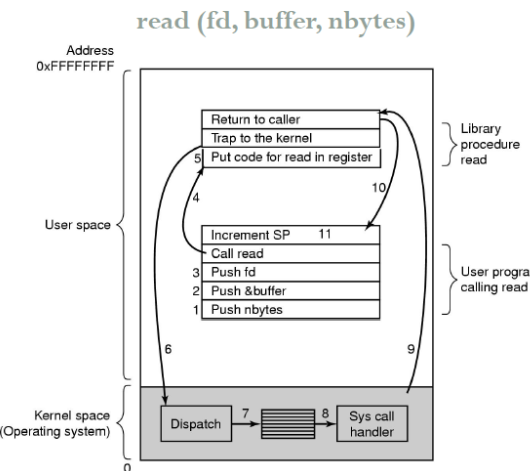
\includegraphics[width=0.3\textwidth]{images/02/stackCall.png}
                        \caption{Passaggio dei parametri tramite \texttt{stack}}
                    \end{figure}
                \subparagraph{Passaggio di parametri tramite tabella} 
                    Come anticipato il passaggio di parametri tramite tabella viene utilizzato per passare parametri complessi o di dimensioni maggiori andando a passare un puntatore alla tabella che contiene i parametri. Questo metodo permette di passare un numero maggiore di parametri e di dimensioni maggiori in quanto i parametri sono passati per riferimento alla memoria primaria.
                    \begin{figure}[H]
                        \centering
                        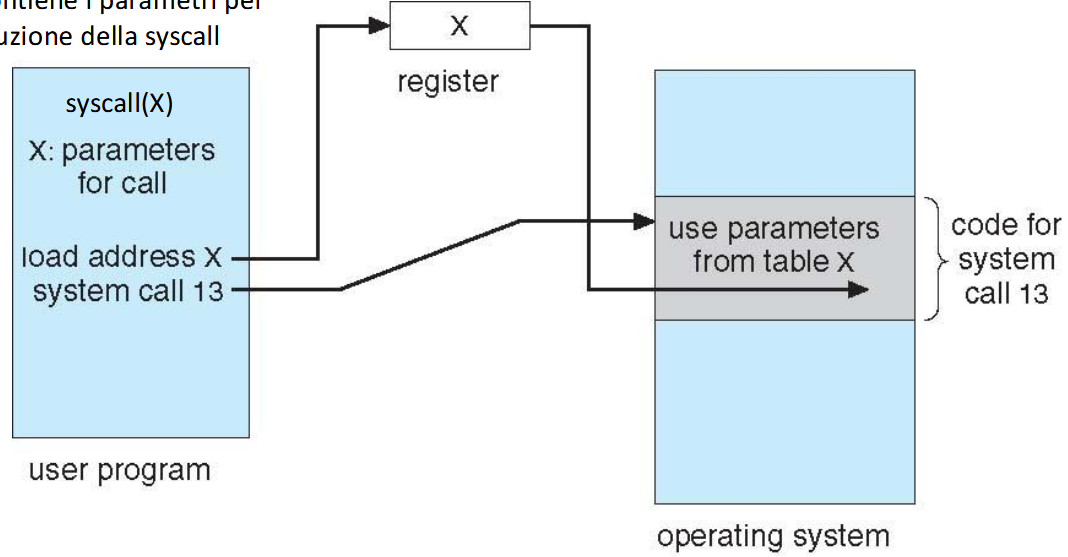
\includegraphics[width=0.3\textwidth]{images/02/tabCall.png}
                        \caption{Passaggio dei parametri tramite tabella}
                    \end{figure}
                    
    \chapter{Architettura di un Sistema Operativo}

In un sistema operativo è molto importante separare le \textit{policy} dai \textit{meccanismi}. I meccanismi sono le funzionalità che il sistema operativo mette a disposizione, mentre le \textit{policy} sono le regole che il sistema operativo segue per decidere come utilizzare i meccanismi.

\paragraph{Principi di progettazione} Il principio di progettazione di un sistema operativo è quello di \texttt{KISS} (\textit{Keep It Small and Simple}) usato per ottimizzare al meglio le \textit{performance} implementando solo lo stretto necessario. Altro principio è il \texttt{POLP} (\textit{Principle of Least Privilege}), ovvero dare il minimo dei privilegi necessari ad ogni componente per svolgere il proprio compito. Quest'ultimo principio è molto importante per garantire affidabilità e sicurezza.

\section{Tipi di architetture}
    \subsubsection{Sistemi monoblocco}
        Nei sistemi monoblocco non è presente una gerarchia tra i vari livelli del sistema operativo. Questo tipo di architettura è molto semplice e consiste in un unico strato \textit{software} tra l'utente ed l'\textit{hardware} del sistema. Le componenti sono dunque tutte allo stesso livello permettendo una comunicazione diretta tra l'utente e l'\textit{hardware}. Questo tipo di architettura è molto semplice e veloce, ma il codice risulta interamente dipendente dall'architettura ed è distribuito su tutto il sistema operativo. Inoltre per testare ed eseguire il \textit{debugging} di un singolo componente è necessario analizzare l'intero sistema operativo.
    \subsubsection{Sistemi a struttura semplice}
        Nei sistemi a struttura semplice è presente una piccola gerarchia, molto flessibile, tra i vari livelli del sistema operativo. Questo tipo di architettura mira ad una riduzione dei costi di sviluppo ed di manutenzione del sistema operativo. Non avendo una struttura ben definita, i componenti possono comunicare tra loro in modo diretto. Questo tipo di architettura è molto flessibile e permette di avere un sistema operativo molto piccolo e veloce come \texttt{MS-DOS} o \texttt{UNIX} originale.
        \paragraph{\texttt{MS-DOS}} Il sistema operativo \texttt{MS-DOS} è un sistema operativo a struttura semplice, molto piccolo e veloce. Questo sistema operativo è pensato per fornire il maggior numero di funzionalità in uno spazio ridotto. Infatti non sussistono suddivisioni in moduli, ed le interfacce e livelli non sono ben definiti. È infatti possibile accedere direttamente alle \textit{routine} del sistema operativo ed non è prevista la \textit{dual mode}.
        \paragraph{\texttt{UNIX} (Originale)} Struttura semplice limitata dalle poche funzionalità disponibili all'epoca in materia di \textit{hardware}, con un \textit{kernel} molto piccolo e veloce il quale scopo è risiedere tra l'interfaccia delle \textit{system call} e l'\textit{hardware}. Questo sistema operativo è stato progettato per essere molto flessibile e fornisce: \textit{File System}, \textit{Scheduling} della \texttt{CPU}, gestione della memoria e molto altro.
        \begin{figure}[H]
            \centering
            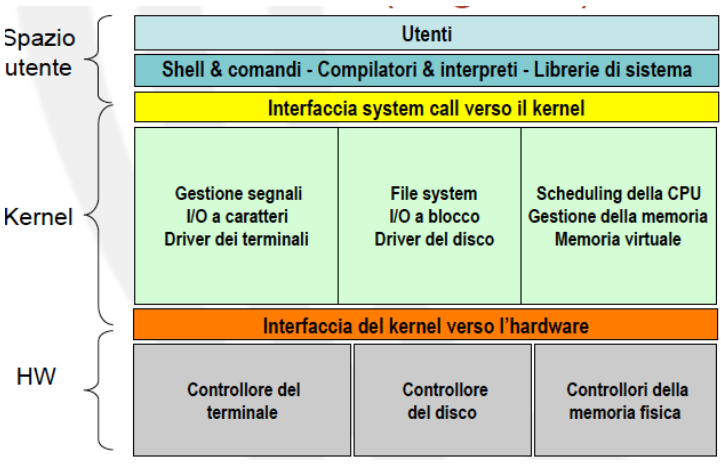
\includegraphics[width=0.6\textwidth]{03/unixOriginal.png}
            \caption{Struttura di \texttt{UNIX} originale}
        \end{figure}
    \subsubsection{Sistema a livelli}
        Nei sistemi operativi organizzati a livelli gerarchici l'interfaccia utente risiede al livello più altro mentre l'\textit{hardware} dal lato opposto. Ogni livello intermedio può solo usare funzioni fornite dal livello inferiore ed offrire funzionalità al livello superiore. Principale vantaggio di questa architettura è la modularità, infatti ogni livello può essere sviluppato e testato indipendentemente dagli altri. Questo tipo di architettura, d'altronde non è priva di svantaggi, infatti diventa difficile definire in modo approssimato gli strati, l'efficienza decresce in quanto ogni singolo strato aggiunge un costo di \textit{overhead} ed le funzionalità dipendenti dal'\textit{hardware} sono sparse su più livelli.
        \paragraph{\texttt{THE}} Il sistema operativo \texttt{THE} è un sistema d'uso accademico ed è il primo sistema operativo a struttura a livelli. Questo \texttt{SO} consiste in un insieme di processo che cooperano tra di loro usando la tecnica dei ``semafori'' per la sincronizzazione. \begin{figure}[H]
            \centering
            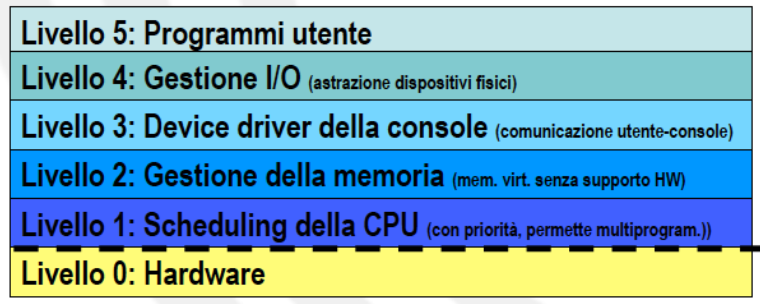
\includegraphics[width=0.4\textwidth]{03/the.png}
            \caption{Struttura di \texttt{THE}}
        \end{figure}
    
    \subsubsection{Sistemi basati su \textit{Kernel}}
        I sistemi di questo genere hanno due soli livelli: i servizi \textit{kernel} e quelli non-\textit{kernel} (o \textit{utente}). Il \textit{file system} è un esempio di servizio non-\textit{kernel}. Questo tipo di architettura è molto diffuso in quanto il ridotto e ben definito numero di livelli ne permette una facile implementazione e manutenzione, spesso però questo sistema può risultare troppo rigido e non adatto a tutti i tipi di applicazioni, oltre alla totale assenza di regole organizzative per le parti del \texttt{SO} al di fuori del \textit{kernel}.
    \subsubsection{\textit{Micro-kenrel}} 
        Questo tipo di \textit{kernel} è molto piccolo e fornisce solo i servizi essenziali per il funzionamento del sistema operativo. Tutte le altre funzionalità sono implementate come processi utente. Un esempio di ciò è \texttt{seL4} un \textit{kernel} \textit{open source} che implementa un \textit{micro-kernel} e fornisce un'interfaccia per la gestione della memoria, dei processi e della comunicazione tra processi. \texttt{SeL4} è matematicamente verificato e privo di bug rispetto alle sue specifiche di forte sicurezza 
    \subsubsection{\textit{Virtual Machine}}
        L'architettura a \texttt{VM} è una estremizzazione dell'approccio a più livelli di \texttt{IBM} (1972), questo è pensato per offrire un sistema di \textit{timesharing} ``multiplo'' dove il sistema operativo viene eseguito su una \texttt{VM} ed questa dà illusione di processi multipli, ma nella realtà ognuno di questi è in esecuzione sul proprio \texttt{HW}. In questo paradigma sono possibili più \texttt{SO} in una unica macchina. 
        \begin{figure}[H]
            \centering
            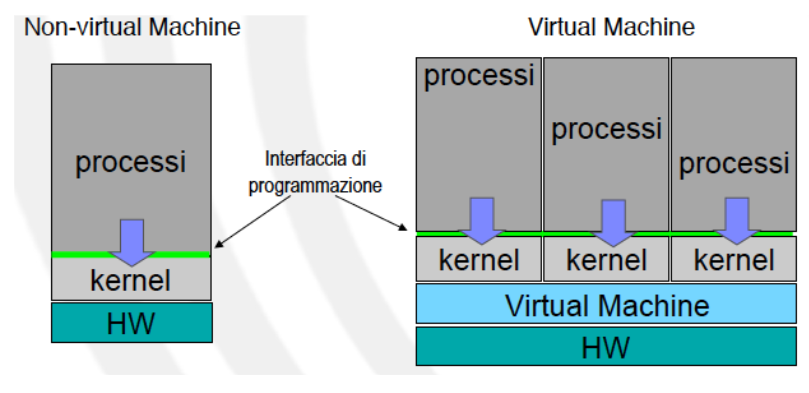
\includegraphics[width=0.4\textwidth]{03/diffVmNoVm.png}
            \caption{Differenze tra una macchina senza e con \texttt{VM}}
        \end{figure}
        Come è possibile notare ogni singolo processo è separato ed possiede il proprio \textit{kernel}. Vengono quindi separata la multiprogrammazione ed la presentazione.
        \paragraph{Tipo di \textit{Hypervisor}}
            \begin{itemize}
                \item \textbf{Tipo 1} (\textit{Bare Metal}): Questo tipo di \textit{Hypervisor} è installato direttamente sul'\textit{hardware} e non necessita di un sistema operativo ospite. Questo tipo di \textit{Hypervisor} è molto veloce e sicuro, ma è molto complesso da installare e configurare.
                \item \textbf{Tipo 2} (\textit{Hosted}): Questo tipo di \textit{Hypervisor} è installato sopra un sistema operativo ospite. Questo tipo di \textit{Hypervisor} è molto più semplice da installare e configurare rispetto al tipo 1, ma è più lento e meno sicuro, inoltre è possibile avere problemi di compatibilità tra il sistema operativo ospite e il \textit{Hypervisor}.
            \end{itemize}
        \paragraph{\textit{Monolithic} vs \textit{Micro-kernel} \texttt{VM}}
            Prima di fare una distinzione tra i due tipi di \texttt{VM} è necessario dire che entrambi rientrano nel tipo 1 di \textit{Hypervisor} e dunque tutti i \texttt{SO} sono eseguiti direttamente sul'\textit{hardware} virtualizzato.
            \begin{itemize}
                \item \textbf{\textit{Monolithic}}: Questo tipo di \texttt{VM} è molto simile ad un sistema operativo tradizionale, infatti ogni \textit{VM} è un processo separato che esegue il proprio \textit{kernel}. Questo tipo di \texttt{VM} è molto veloce, ma è molto complesso da implementare e mantenere.
                \item \textbf{\textit{Micro-kernel}}: Questo tipo di \texttt{VM} è molto simile ad un sistema operativo a \textit{micro-kernel}, infatti il \textit{kernel} della \texttt{VM} fornisce solo i servizi essenziali per il funzionamento del sistema operativo. Tutte le altre funzionalità sono implementate come processi utente. Questo tipo di \texttt{VM} è molto più semplice da implementare e mantenere rispetto al tipo 1, ma è più lento e meno sicuro.
            \end{itemize}
        \paragraph{Vantaggi - Svantaggi}
            Principale vantaggio di questo tipo di architettura è la completa protezione del sistema, infatti ogni \texttt{SO} è separato e non può accedere alle risorse degli altri \texttt{SO}. Inoltre è possibile avere più \texttt{SO} in una sola macchina andando ad ottimizzare le risorse e ridurre i costi di sviluppo di un sistema operativo, oltre ad aumentare la portabilità delle applicazioni. Principale svantaggio riguardano le prestazioni del sistema, infatti ogni \texttt{SO} è eseguito su una \texttt{VM} e questo può portare ad un aumento dei tempi di esecuzione delle applicazioni. Inoltre è necessario avere gestire una \textit{dual-mode} virtuale e non è possibile avere un sistema operativo in tempo reale, inoltre il fatto che una \texttt{VM} non possa accedere alle altre \texttt{VM} può portare ad un aumento dei costi di sviluppo e manutenzione del sistema.
    \subsubsection{Sistemi \textit{client-server}}
        Poco diffusi ai giorni nostri, i sistemi \textit{client-server} sono basati su un'architettura a due livelli: il \textit{client} e il \textit{server}. Questo sistema di basa sull'idea che il codice del sistema operativo vada portato sul livello superiore (il \textit{client}) e il \textit{server} rimanga molto piccolo e veloce andando solo a fornire i servizi essenziali per il funzionamento del sistema operativo ed la comunicazione tra il \textit{client} e l'\textit{hardware}. Questo tipo di architettura si presta bene per sistemi distribuiti.
\section{Implementazione di un \texttt{SO}}
    I sistemi operativi sono tradizionalmente scritti in linguaggio \textit{assembler} anche se è possibile scriverli in linguaggi di alto livello, come \texttt{C} o \texttt{C++}. La scrittura di un sistema operativo in linguaggio di alto livello permette di avere una implementazione molto rapida oltre ad aumentarne la compattezza e la mantienebilità. Inoltre è possibile avere una maggiore portabilità del sistema operativo, in quanto è possibile compilare il codice sorgente su più architetture. Tuttavia la scrittura di un sistema operativo in linguaggio di alto livello può portare ad un aumento dei tempi di esecuzione delle applicazioni e ad un aumento dei costi di sviluppo e manutenzione del sistema operativo. 
    \chapter{Processi e \textit{Thread}}

In questo capitolo vedremo cosa sono i processi e i \textit{thread} capendone le differenze e le somiglianze, vedremo come vengono gestiti e come vengono eseguiti. Infine vedremo come vengono gestiti i processi dal sistema operativo e come vengono eseguiti i processi dal sistema operativo.

\section{Processi}
    Un processo è l'istanza di un programma in esecuzione, quando il programma viene eseguito e quindi caricato nella memoria primaria (\texttt{RAM}) diventa un processo. Mentre un programma è la parte statica di un software, il processo è la parte dinamica. Un processo viene eseguito in maniera sequenziale, ovvero un'istruzione alla volta, ma nei sistemi operativi moderni un processo può essere eseguito in maniera concorrente, ovvero più processi possono essere eseguiti in parallelo.
    \subsubsection{Immagine in memoria}
        Un processo quando viene caricato in memoria viene caricato in una zona di memoria chiamata \textit{spazio degli indirizzi} (\textit{address space}). Questo spazio è diviso in varie sezioni (da indirizzi alti ad indirizzi bassi):
        \begin{itemize}
            \item \textbf{Dati}: contiene le variabili globali e statiche del programma.
            \item \textbf{\textit{Stack}}: contiene le variabili locali e i parametri delle funzioni.
            \item eventuale memoria dinamica allocata durante l'esecuzione.
            \item \textbf{\textit{Heap}}: contiene la memoria dinamica allocata durante
            \item \textbf{Codice}: contiene il codice del programma.
            \item \textbf{Attributi del processo}: contiene informazioni sul processo.
        \end{itemize}
    \subsection{Stato di un processo}
        Un processo durante la sua creazione ed esecuzione può trovarsi in diversi stati:
        \begin{itemize}
            \item \textbf{Nuovo}: il processo è stato creato ma non è ancora in esecuzione.
            \item \textbf{Pronto}: il processo è pronto per essere eseguito, ma non è ancora in esecuzione. (oppure è stato messo in attesa dalla \texttt{CPU}).
            \item \textbf{In esecuzione}: il processo è in esecuzione sulla \texttt{CPU}.
            \item \textbf{In attesa}: il processo è in attesa di un evento (es. \texttt{I/O}).
            \item \textbf{Terminato}: il processo è terminato.
        \end{itemize}
        Per la gestione di questi stati il sistema operativo usa un \textit{dispatcher} il quale compito è quello di passare tra i processi e cambiare il loro stato. Per questo motivo il \textit{dispatcher} è chiamato anche \textit{scheduler}.
        \subsubsection{\textit{Scheduling}}
        \label{sec:scheduling04}
            Lo \textit{scheduling} è il processo di selezione del processo da eseguire sulla \texttt{CPU}. Esistono vari tipi di \textit{scheduler}:
            \begin{itemize}
                \item \textbf{\textit{Long time scheduler}}: decide quali processi devono essere caricati in memoria. (Nella coda dei processi pronti).
                \item \textbf{\textit{Short time scheduler}}: decide quale processo deve essere eseguito sulla \texttt{CPU}. (Seleziona i processi dalla coda dei processi pronti).
            \end{itemize}
            Mentre lo \textit{short-term} scheduler è un processo molto veloce in quanto viene chiamato molto spesso (ogni $10-100 ms$), il \textit{long-term} scheduler è un processo più lento in quanto viene chiamato molto raramente (ogni $1-10 s$ o anche di più), questo però è responsabile del grado di multiprogrammazione del sistema. 
            \paragraph{Accantonamento}
                L'accantonamento è il processo per il quale i processi pronti ad essere eseguiti vengono messi in una coda di attesa. Quando la \texttt{CPU} è pronta per eseguire un processo, il processo viene preso dalla coda e viene eseguito, nel caso nel quale il processo richieda un'operazione di \texttt{I/O} il processo viene messo in richiesta ed quando l'operazione di \texttt{I/O} (caratterizzata a sua volta da una coda per ogni dispositivo connesso) è completata il processo viene rimesso nella coda dei processi pronti.\newline 
                Può anche succedere che il tempo per l'esecuzione di un processo sia scaduto, in questo caso il processo viene rimesso nella coda dei processi pronti. Se poi il processo generi dei processi figli, questi dopo la loro inizializzazione vengono messi nella coda dei processi pronti e vengono eseguiti, se il padre necessita che il processo figlio termini prima di lui, il padre viene messo in attesa che il figlio termini, altrimenti anche il padre viene messo nella coda dei processi pronti. Infine se un processo necessita di un segnale da parte di un altro processo, il processo viene messo in attesa finché non riceve il segnale (dal sistema o da un altro processo).
            \paragraph{\texttt{I/O} vs \texttt{CPU} \textit{bound}}
                Un processo può essere \texttt{I/O} bound o \texttt{CPU} \textit{bound}. Un processo \texttt{I/O} \textit{bound} è un processo che richiede molte operazioni di \texttt{I/O} e poche operazioni sulla \texttt{CPU}, mentre un processo \texttt{CPU} \textit{bound} è un processo che richiede molte operazioni sulla \texttt{CPU} e poche operazioni di \texttt{I/O}. Non è possibile stabilire a priori se un processo è \texttt{I/O} \textit{bound} o \texttt{CPU} \textit{bound}, ma è possibile stabilirlo solo durante l'esecuzione del processo analizzando quanta \texttt{CPU} usa e se richiede molte operazioni di \texttt{I/O}, sulla base di questo il processo viene classificato come \texttt{I/O} \textit{bound} o \texttt{CPU} \textit{bound}.
        \subsubsection{Operazione di \textit{dispatch}}
            Quando si deve passare da un processo ad un altro si deve fare un'operazione di \textit{dispatch}. Questa operazione consiste nel:
            \begin{enumerate}
                \item Cambiare il contesto (salvare lo stato del processo corrente (\texttt{PCB}) e caricare lo stato del processo successivo (\texttt{PCB})).
                \item Passare alla modalità utente (quando viene eseguito il \textit{context switch} il sistema operativo è in modalità \textit{kernel}, mentre il processo deve essere eseguito in modalità utente).
                \item Salto alla prossima istruzione da eseguire del processo successivo.
            \end{enumerate}
            Questa operazione è molto costosa in termini di tempo, in particolare l'operazione di \textit{context switch} richiede risorse che rallentano il sistema senza eseguire nessuna operazione utile, la durata di ciò è strettamente dipendente dall'architettura del processore e dal sistema operativo.
    \subsection{Operazioni sui processi}
        Nella quasi totalità dei sistemi operativi moderni è possibile eseguire più processi in parallelo, per fare ciò il sistema operativo deve fornire delle operazioni per la gestione dei processi oltre ad un modo per l'identificazione dei processi. Di seguito vediamo quali sono le operazioni possibili sui processi.
        \subsubsection{Creazione di un processo}
            Un processo, come già detto, può creare altri processi, questi processi creati sono detti processi figli. Un processo padre può creare più processi figli, questi processi figli possono creare a loro volta altri processi figli e così via. Ai processi normalmente viene associato un \textit{PID} (\textit{Process IDentifier}) che è un numero univoco che identifica il processo all'interno del sistema operativo. \newline
            Il processo figlio può ottenere le risorse necessarie per la sua esecuzione in due modi:
            \begin{itemize}
                \item Ereditando le risorse del processo padre (\textit{sharing})
                \item Ottenendo nuove risorse dal sistema operativo (\textit{partitioning})
            \end{itemize}
            Inoltre il processo figlio può essere eseguito in parallelo in maniera sincrona rispetto al processo padre (il processo padre aspetta che il processo figlio termini) o asincrona (il processo figlio viene eseguito in parallelo al processo padre).
            \paragraph{Nei sistemi \texttt{UNIX}} Nei sistemi \texttt{UNIX} esistono diverse \textit{system call} per la creazione di processi, la principale è \texttt{fork()} che crea un processo figlio identico al processo padre, la differenza tra i due processi è il \textit{PID} e il \textit{PPID} (\textit{Parent Process IDentifier}). Il processo figlio eredita tutte le risorse del processo padre, inoltre il processo figlio può modificare le risorse ereditate dal processo padre. Altra chiamata di sistema è \texttt{exec()} che permette di caricare un nuovo programma in un processo figlio, in questo caso il programma tra il processo padre e il processo figlio è differente. Infine la chiamata di sistema \texttt{wait()} permette l'esecuzione sincrona di un processo figlio rispetto al processo padre.
        \subsubsection{Terminazione di un processo}
            Un processo può terminare in tre modi:
            \begin{itemize}
                \item \textbf{Normalmente}: il processo termina la sua esecuzione invocando la \textit{system call} \texttt{exit()} (con eventualmente un codice di uscita).
                \item \textbf{Forzatamente dal processo padre}: il processo padre può terminare il processo figlio invocando la \textit{system call} \texttt{kill()}, oppure nel caso di un eccessivo uso di risorse, oppure a sua volta il processo padre termina anormalmente.
                \item \textbf{Forzatamente dal sistema operativo}: il sistema operativo può terminare un processo nel caso di un errore di esecuzione, oppure nel caso nel quale l'utente chiuda l'applicazione.
            \end{itemize}
            Nota come nel primo caso non sia esclusa la possibilità che il processo termini in maniera anomala, ad esempio per un errore di esecuzione gestito dal processo stesso, infatti quando il codice di uscita è diverso da \texttt{0} si intende che il processo è terminato in maniera anomala, ogni codice diverso da \texttt{0} ha un significato diverso.\newline
            Quando un processo termina il sistema operativo si occupa di liberare le risorse utilizzate dal processo come la memoria allocata, i file aperti, le connessioni di rete, o altre risorse.
    \subsection{Gestione dei processi del \texttt{SO}}
        Di fatto il sistema operativo non è altro che un programma a tutti gli effetti, e dunque la sua esecuzione è un processo come un altro. Questo non significa però che il sistema operativo non essere gestito separatamente dagli altri processi, infetti esistono diverse opzioni l'esecuzione del \textit{kernel}:
        \begin{itemize}
            \item Il \textit{kernel} viene eseguito completamente in maniera separata dagli altri processi.
            \item Il \textit{kernel} viene eseguito all'interno di un processo utente.
            \item Il \textit{kernel} viene eseguito come un processo separato.
        \end{itemize}
        \paragraph{\textit{Kernel} separato} In questo caso il \textit{kernel} è eseguito al di fuori degli altri processi, questo gli permette di avere uno spazio in memoria ben definito e riservato oltre ad avere il totale controllo del sistema ed a essere eseguito in modalità \textit{kernel} (ovvero con privilegi elevati). I processi sono dunque solo propri all'utente ed un processo non potrà mai essere eseguito in modalità \textit{kernel}.
        \paragraph{\textit{Kernel} nel processo utente} In questo caso il \textit{kernel} è eseguito all'interno di un processo utente, questo permette ai programmi utente di chiamare qualunque servizio del sistema operativo, ma tramite una modalità protetta (\textit{kernel mode}) che permette al sistema operativo di controllare le chiamate e di evitare che un processo utente possa fare danni al sistema. Dato che il \textit{kernel} è un processo a tutti gli effetti la sua immagine in memoria sarà composta dal ``\textit{kernel stack}'' per la gestione delle chiamate di sistema e dal ``\textit{kernel code}'' che consiste nei dati e codice del \texttt{SO} condiviso tra tutti i processi.\newline
        Questo approccio porta ad una riduzione del tempo di \textit{context switch} in quanto è necessario solo la \textit{mode switch} e non l'intero \textit{context switch} lasciando però intatte le possibilità di riattivazione del processo utente o di eseguire un altro processo eseguendo un \textit{context switch} completo.
        \paragraph{\textit{Kernel} come processo separato} In questo caso ogni servizio del sistema operativo è eseguito come un processo separato in modalità protetta. L'unica parte del \textit{kernel} che deve essere eseguita separatamente è lo \textit{scheduler} in quanto deve essere eseguito in modalità \textit{kernel}. Questo approccio è molto vantaggioso per sistemi multiprocessore in quanto permette di eseguire i servizi del sistema operativo in parallelo ed in un processore designato.
\section{\textit{Thread}}
    Un \textit{thread} è l'unità di base d'uso della \texttt{CPU}, un processo può contenere uno o più \textit{thread} che condividono lo stesso codice, dati e file aperti, ma ognuno ha un suo \textit{stack}, lo stato del \textit{program counter} e dei registri ed un numero identificativo.\newline
    Dunque le risorse e lo spazio di indirizzamento sono propri del processo, mentre lo stato della \texttt{CPU} è proprio del \textit{thread} assieme al \textit{program counter} e ai registri.\newline
    Classicamente un processo è composto da un solo \textit{thread}, la capacità di avere più \textit{thread} in un processo è chiamata \textit{multithreading}. Questo permette di avere un processo con più \textit{thread} separando il flusso di esecuzione e lo spazio di indirizzamento, ma condividendo le risorse del processo. 
    \paragraph{Vantaggi}
        I vantaggi del \textit{multithreading} sono:
        \begin{itemize}
            \item \textbf{Risposta più veloce}: Se sono necessari molti calcoli o operazioni di \texttt{I/O} è possibile eseguire queste operazioni in parallelo.
            \item \textbf{Condivisione delle risorse}: I \textit{thread} possono condividere le risorse del processo, mentre processi separati devono usare meccanismi di comunicazione.
            \item \textbf{Economia}: Creare un \textit{thread} è più veloce e meno costoso di creare un processo.
            \item \textbf{Scalabilità}: I \textit{thread} possono essere eseguiti in parallelo su più processori o su più core.
        \end{itemize}
    \subsection{Implementazione dei \textit{thread}}
        Vediamo ora come sono implementati i \textit{thread} nei sistemi operativi.
        \subsubsection{Stato dei \textit{thread}}
            Un \textit{thread}, come un processo, può trovarsi in diversi stati:
            \begin{itemize}
                \item \textbf{Pronto}: il \textit{thread} è pronto per essere eseguito.
                \item \textbf{In esecuzione}: il \textit{thread} è in esecuzione sulla \texttt{CPU}.
                \item \textbf{In attesa}: il \textit{thread} è in attesa di un evento.
            \end{itemize}
            Un \textit{thread} può essere in uno di questi stati, ma il processo può non essere nello stesso stato di un \textit{thread} in quanto un processo può contenere più \textit{thread} e quindi un processo può essere in uno stato diverso da quello dei suoi \textit{thread}.\newline
            Un classico problema degli stati dei \textit{thread} è la questione di cosa fare quando un \textit{thread} è in attesa di un evento, questa ``attesa'' deve bloccare l'intero processo o solo il \textit{thread} in attesa? Ciò dipende dall'implementazione dei \textit{thread} nel sistema operativo.
        \subsubsection{Implementazione dei \textit{thread}}
            Esistono due principali implementazioni dei \textit{thread}:
            \begin{itemize}
                \item \textbf{\textit{User-level threads}}: I \textit{thread} sono implementati a livello utente, il sistema operativo non è a conoscenza dei \textit{thread} e non li gestisce. Le funzionalità sono implementate in una libreria che gestisce i \textit{thread} e le chiamate di sistema.
                \item \textbf{\textit{Kernel-level threads}}: I \textit{thread} sono implementati a livello del \textit{kernel}, il sistema operativo è a conoscenza dei \textit{thread} e li gestisce. 
                \item \textbf{\textit{Hybrid threads}}: I \textit{thread} sono implementati a livello del \textit{kernel}, ma il sistema operativo permette di creare \textit{thread} a livello utente. (es. \texttt{SOLARIS})
            \end{itemize}
            \paragraph{\textit{User-level threads}} Se si opta per l'implementazione dei \textit{thread} a livello utente, il sistema operativo non è a conoscenza dei \textit{thread} e non li gestisce e dunque non è necessario passare in modalità \textit{kernel} per la gestione dei \textit{thread} risparmiando due \textit{context switch}. Ogni applicazione deve però implementate lo \textit{scheduler} dei \textit{thread} e la gestione degli stati dei \textit{thread}. Quanto detto garantisce una maggiore portabilità delle applicazioni senza dover riscrivere il codice per ogni sistema operativo, ma allo stesso tempo non permette di sfruttare appieno le potenzialità del sistema operativo. Se però un \textit{thread} necessita di un'operazione di \texttt{I/O} o di un'operazione che richiede l'intervento del sistema operativo, tutti i \textit{thread} del processo vengono bloccati in quanto il sistema operativo non è a conoscenza dei \textit{thread} e non può gestire i \textit{thread} in maniera indipendente. (es. \textit{Green threads (\texttt{JDK1.1})}, \texttt{GNU} \textit{Portable Threads}, \texttt{POSIX} \textit{Pthreads})
            \paragraph{\textit{Kernel-level threads}} Se si opta per l'implementazione dei \textit{thread} a livello del \textit{kernel}, il sistema operativo è a conoscenza dei \textit{thread} e li gestisce, dunque il sistema operativo può gestire i \textit{thread} in maniera indipendente e può sfruttare appieno le potenzialità del sistema operativo. Ogni \textit{thread} è un processo a tutti gli effetti, dunque ogni \textit{thread} ha il proprio \textit{PCB} e il proprio spazio di indirizzamento. Questo permette di sfruttare appieno le potenzialità del sistema operativo, ma allo stesso tempo richiede due \textit{context switch} per passare da un \textit{thread} all'altro. (es. \texttt{Windows}, \texttt{Linux}, \textit{Native Threads (\texttt{JDK1.2})})
            \paragraph{\textit{Hybrid threads}} Se si opta per l'implementazione dei \textit{thread} ibridi, il sistema operativo permette di creare \textit{thread} a livello utente, ma i \textit{thread} sono implementati a livello del \textit{kernel}. Questo permette di sfruttare appieno le potenzialità del sistema operativo, ma allo stesso tempo permette di creare \textit{thread} a livello utente. (es. \texttt{SOLARIS})
    \subsection{Esempio di libreria - \texttt{pthreads}}
        Nel caso di implementazione dei \textit{thread} a livello utente, il sistema operativo non è a conoscenza dei \textit{thread} e dunque non li gestisce, ma è necessario utilizzare una libreria che gestisca i \textit{thread}. Un esempio di libreria per la gestione dei \textit{thread} è \texttt{pthreads} (\texttt{POSIX} \textit{Threads}).\newline
        \texttt{pthreads} è una libreria standard per la gestione dei \textit{thread} in sistemi \texttt{UNIX} e sistemi \texttt{UNIX-like}. La libreria fornisce un'interfaccia standard per la creazione, la sincronizzazione e la terminazione dei \textit{thread} nel linguaggio \texttt{C}. La libreria fornisce la possibilità di caratterizzare i \textit{thread} sulla base della priorità (influenza lo \textit{scheduling}) e della dimensione dello \textit{stack} (stabilisce quante risorse può utilizzare il \textit{thread}).\newline
        Gli attributi di un \textit{thread} sono contenuti nell'oggetto di tipo \texttt{pthread\_attr\_t} e tramite la funzione \texttt{pthread\_attr\_init()} si inizializzano gli attributi del \textit{thread}. Una volta inizializzati gli attributi tramite la funzione \texttt{pthread\_create()} si crea il \textit{thread} passando come argomenti:
        \begin{enumerate}
            \item Una variabile del tipo \texttt{pthread\_t} che conterrà l'identificativo del \textit{thread}.
            \item Un oggetto del tipo \texttt{pthread\_attr\_t} che conterrà gli attributi del \textit{thread}.
            \item Un puntatore alla funzione che il \textit{thread} dovrà eseguire.
            \item Un puntatore agli argomenti della funzione.
        \end{enumerate}
        Una volta creato il \textit{thread} questo terminerà quando il codice della funzione terminerà, oppure quando nel codice della funzione verrà invocata la funzione \texttt{pthread\_exit()} con parametro \texttt{value\_ptr} che conterrà il valore di uscita del \textit{thread}. Se invece il \textit{thread} deve essere sospeso in attesa di un altro \textit{thread} si può utilizzare la funzione \texttt{pthread\_join()} con parametri:
        \begin{enumerate}
            \item Un oggetto del tipo \texttt{pthread\_t} che identifica il \textit{thread} da attendere.
            \item Un puntatore alla variabile che conterrà il valore di uscita del \textit{thread} atteso.
        \end{enumerate}
\begin{lstlisting}[language=C]
#include <pthread.h>
#include <stdio.h>
void *tbody(void *arg)
    {
    int j;
    printf("ciao sono un thread, mi hanno appena creato\n");
    *(int *)arg = 10;
    sleep(2) /* faccio aspettare un po il mio creatore poi termino */
    pthread_exit((int *)50); /* oppure return ((int *)50); */
}
main(int argc, char **argv)
{
    int i;
    pthread_t mythread;
    void *result;
    printf("sono il primo thread, ora ne creo un altro \n");
    pthread_create(&mythread, NULL, tbody, (void *) &i);
    printf("ora aspetto la terminazione del thread che ho creato \n");
    pthread_join(mythread, &result);
    printf("Il thread creato ha assegnato %d ad i\n",i);
    printf("Il thread ha restituito %d \n",result);
}
\end{lstlisting}
    In questo esempio la variabile ``mythread'' assume dei valori corrispondenti all'identificativo del \textit{thread} creato, mentre la variabile ``result'' assume il valore di uscita del \textit{thread} creato. La funzione ``tbody'' è la funzione che il \textit{thread} dovrà eseguire, mentre la variabile ``i'' è un argomento passato alla funzione. La funzione ``pthread\_exit()'' termina il \textit{thread} e restituisce il valore passato come argomento, mentre la funzione ``pthread\_join()'' sospende il \textit{thread} corrente in attesa del \textit{thread} passato come argomento e restituisce il valore di uscita del \textit{thread} atteso.
    \subsubsection{Condivisione dello spazio logico} 
        Come già anticipato i \textit{thread} condividono lo stesso spazio logico, questo significa che i \textit{thread} possono accedere alle stesse variabili globali e statiche e se un \textit{thread} modifica una variabile globale, la modifica sarà visibile a tutti gli altri \textit{thread}. Questo può portare a problemi di sincronizzazione tra i \textit{thread} e dunque è necessario utilizzare meccanismi di sincronizzazione per evitare problemi di accesso concorrente alle variabili globali. Possono esistere variabili locali ai \textit{thread} che sono visibili solo al \textit{thread} che le ha dichiarate, ma non sono visibili agli altri \textit{thread}, ciò usando la classe \texttt{thread\_specific\_data}.
        \paragraph{Per la sincronizzazione} Per la sincronizzazione tra i \textit{thread} si possono utilizzare o gli strumenti direttamente forniti dalla libreria \texttt{pthreads} (come i semafori) oppure si possono utilizzare le primitive di sincronizzazione fornite dal sistema operativo (come \texttt{sleep(n)} che sospende il \textit{thread} corrente per $n$ secondi). Per tenere traccia del tempo trascorso nella funzione possono essere usati due metodi:
        \begin{itemize}
            \item Un \textit{interrupt Request} (\texttt{IRQ}) che viene generato ad intervalli regolari e che incrementa un contatore. Il \texttt{SO} controlla se ci sono delle \texttt{sleep} scadute e se ci sono le risveglia.
            \item Riconfigurazione delle \texttt{IRQ} in modo che avvenga una \texttt{IRQ} quando la prima \texttt{sleep} scade, e una seconda \texttt{IRQ} quando la seconda \texttt{sleep} scade e così via. Ciò comporta a migliore precisione ma alto \textit{overhead} per la riconfigurazione delle \texttt{IRQ} ad ogni \texttt{sleep}.
        \end{itemize}
    \chapter{Comunicazione tra processi}

Normalmente i processi si dividono in processi indipendenti, ovvero quei processi la cui esecuzione è indipendente da quella degli altri processi ed non condivide i dati, e processi cooperanti, ovvero quei processi che condividono i dati e devono comunicare tra loro, la loro esecuzione non è deterministica e non è riproducibile.
\paragraph{In generale}
    Esistono diversi motivi per cui i processi devono comunicare tra loro, tra cui:
    \begin{itemize}
        \item \textbf{Scambio di informazioni}: i processi devono scambiarsi informazioni per cooperare tra loro.
        \item \textbf{Accelerazione del calcolo}: i processi possono cooperare per eseguire un calcolo più velocemente.
        \item \textbf{Modularità}: i processi possono essere scritti in modo indipendente e comunicare tra loro per cooperare.
        \item \textbf{Convenienza}: è più semplice scrivere processi separati che cooperano tra loro piuttosto che scrivere un unico processo.
    \end{itemize}
    per ottenere una comunicazione tra processi è necessario che i processi condividano un canale di comunicazione, esistono due tipi di canali di comunicazione:
    \begin{description}
        \item[scambio di messaggi] i processi comunicano scambiandosi messaggi che vengono inviati attraverso un canale di comunicazione tra il \textit{kernel} e i processi, i messaggi possono essere inviati in modo sincrono o asincrono.
        \item[memoria condivisa] i processi comunicano condividendo una regione di memoria, i processi possono leggere e scrivere nella memoria condivisa, la memoria condivisa è un canale di comunicazione molto più veloce rispetto allo scambio di messaggi, ma è più difficile da gestire.
    \end{description}
    Il primo risulta più sicuro in quanto i processi non possono accedere direttamente alla memoria degli altri processi ed il messaggio viene verificato dal \textit{kernel} prima di essere inviato, mentre il secondo è più veloce in quanto non richiede l'intervento del \textit{kernel} per la comunicazione.\newline
    Tutti i meccanismi di comunicazione tra processi sono implementati dal \textit{kernel} del sistema operativo racchiusi nei protocolli di comunicazione tra processi (\texttt{IPC} - \textit{Inter-Process Communication}).

\section{\texttt{IPC} - \textit{Message Passing}}
    Il protocollo \texttt{ICP} racchiude un insieme di meccanismi che permettono la comunicazione tra processi, tra i quali vi è il \textit{message passing}, ovvero un meccanismo che permette ai processi di comunicare scambiandosi messaggi e senza condividere delle variabili e/o memoria. Le operazioni di base che ogni \texttt{SO} deve fornire per il \textit{message passing} sono:
    \begin{itemize}
        \item \texttt{send} - invia un messaggio ad un processo. (con lunghezza fissa o variabile)
        \item \texttt{receive} - riceve un messaggio da un processo.
    \end{itemize}
    Prima ancora che i processi possano comunicare tra loro è necessario che essi siano in grado di identificarsi e stabilire un canale di comunicazione, per fare ciò è necessario che i processi abbiano un identificativo univoco, ovvero un \textit{PID} (\textit{Process IDentifier}).\newline
    L'implementazione di questo canale di comunicazione può essere realizzata in due modi:
    \begin{description}
        \item[livello fisico] i messaggi vengono inviati attraverso un canale di comunicazione fisico, come ad esempio una rete o un bus.
        \item[livello logico] i messaggi vengono inviati attraverso un canale di comunicazione logico, come ad esempio una coda di messaggi.
    \end{description}
    Le scelte di uno o dell'altro canale di comunicazione dipendono dalle esigenze del sistema e dalle prestazioni richieste. Fattori che influenzano la scelta sono:
    \begin{itemize}
        \item Come vengono stabiliti i canali
        \item Se un canale può essere utilizzato da più processi contemporaneamente
        \item Quanti canali possono essere aperti contemporaneamente tra una stessa coppia di processi
        \item La lunghezza massima del canale
        \item La lunghezza (fissa/variabile) massima dei messaggi
        \item Se il canale è \textit{simplex}, \textit{half-duplex} o \textit{full-duplex}
    \end{itemize}
    \subsection{Nominazione}
        A livello di nominazione, ovvero come i processi si identificano, esiste la comunicazione diretta e la comunicazione indiretta:
        \subsubsection{Comunicazione Diretta}
            Nella comunicazione diretta i processi si identificano direttamente, ovvero il mittente conosce l'identificativo del destinatario e viceversa, in questo modo il mittente può inviare il messaggio direttamente al destinatario. Questo metodo è molto veloce, ma presenta dei problemi:
            \begin{itemize}
                \item Il mittente deve conoscere l'identificativo del destinatario
                \item Il destinatario deve essere in esecuzione
                \item Nel caso in cui il destinatario o il ricevente cambi identificativo, il mittente deve essere aggiornato
            \end{itemize}
            La comunicazione diretta può a sua volta essere simmetrica o asimmetrica:
            \begin{description}
                \item[Simmetrica] Il mittente e il destinatario si conoscono a priori e possono comunicare tra loro. Sia per l'invio che per la ricezione dei messaggi è necessario conoscere l'identificativo del processo con cui si vuole comunicare.
                \item[Asimmetrica] Il mittente e il destinatario non si conoscono a priori. Solo il mittente conosce l'identificativo del destinatario, il destinatario non conosce l'identificativo del mittente ed ascolta qualsiasi messaggio che arriva.
            \end{description}
        \subsubsection{Comunicazione Indiretta}
            Nella comunicazione indiretta i messaggi vengono inviati ad un canale di comunicazione comune detto \textit{mailbox} (o porte), ognuna di queste \textit{mailbox} ha associato un numero identificativo univoco, i processi possono inviare e ricevere messaggi da queste \textit{mailbox} senza dover conoscere l'identificativo del destinatario, ma devono condividere una \textit{mailbox} comune.
            \paragraph{Flusso di una \textit{mailbox}}
                Prima di poter inviare un messaggio ad una \textit{mailbox} è necessario che questa venga creata, una volta creata la \textit{mailbox} il processo può inviare un messaggio ad essa, il messaggio viene inserito in una coda di messaggi associata alla \textit{mailbox}, il destinatario può ricevere il messaggio dalla \textit{mailbox} e leggerlo, una volta letto il messaggio viene rimosso dalla coda. Quando la \textit{mailbox} non è più necessaria può essere eliminata.
            \paragraph{Invio e ricezione} 
                Per inviare e ricevere messaggi da una \textit{mailbox} è necessario conoscere l'identificativo della \textit{mailbox}, una volta conosciuto l'identificativo il processo può inviare e ricevere messaggi dalla \textit{mailbox}.
            \paragraph{Proprietà del canale} Come già detto, il canale di comunicazione viene stabilito solo se i processi condividono una \textit{mailbox}, ma una \textit{mailbox} può essere associata a molti processi ed una stessa coppia di processi può avere più \textit{mailbox} associate, inoltre una \textit{mailbox} può essere o meno bi-direzionale.
            \paragraph{Problema riceventi multipli} Un problema che si può presentare è quello dei riceventi multipli, ovvero quando un mittente invia un messaggio ad una \textit{mailbox} e ci sono più processi che ricevono i messaggi da quella \textit{mailbox}, in questo caso il \textit{SO} deve permettere solo ad uno dei processi di ricevere il messaggio, e questo viene fatto in maniera arbitraria.
    \subsection{Sincronizzazione} 
        Uno scambio di messaggi può essere ``bloccante'' (sincrono) o ``non bloccante'' (asincrono), ovvero il mittente può continuare ad eseguire il proprio codice dopo aver inviato il messaggio o deve attendere che il destinatario riceva il messaggio.\newline
        Se il canale di comunicazione è bloccante, il mittente deve attendere che il destinatario riceva il messaggio ed assicurarsi che il messaggio sia stato ricevuto, se il canale di comunicazione è non bloccante il mittente può continuare ad eseguire il proprio codice dopo aver inviato il messaggio, senza dover attendere che il destinatario riceva il messaggio, in questo caso il mittente non può sapere se il messaggio è stato ricevuto o meno.
        \begin{figure}[H]
            \begin{subfigure}{0.45\textwidth}
                \centering
                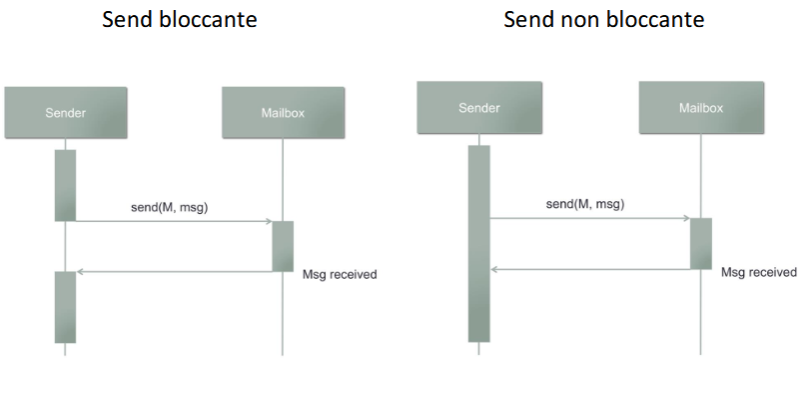
\includegraphics[width=\textwidth]{05/send.png}
                \caption{Invio bloccante/non bloccante}
            \end{subfigure}
            \begin{subfigure}{0.45\textwidth}
                \centering
                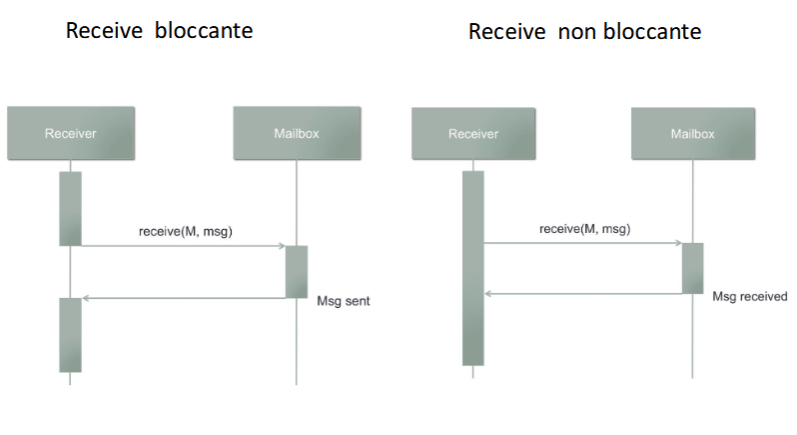
\includegraphics[width=\textwidth]{05/receive.png}
                \caption{Ricezione bloccante/non bloccante}
            \end{subfigure}
            \caption{Invio e ricezione bloccante/non bloccante}
        \end{figure}

\section{\texttt{IPC} - Memoria Condivisa}
    Un altro meccanismo di comunicazione tra processi è la memoria condivisa, ovvero un'area di memoria condivisa tra più processi, i processi possono leggere e scrivere nella memoria condivisa, la memoria condivisa è un canale di comunicazione molto più veloce rispetto allo scambio di messaggi, ma è più difficile da gestire, inoltre il \textit{kernel} non può controllare l'accesso alla memoria condivisa, quindi è necessario che i processi si sincronizzino tra loro per evitare problemi di accesso concorrente.
    \subsubsection{Flusso di \texttt{POSIX}}
        Prendiamo come esempio la memoria condivisa in \texttt{POSIX}, per poter utilizzare la memoria condivisa è necessario che uno dei processi crei la memoria condivisa, una volta creata la memoria condivisa l'altro processo deve ``attaccarsi'' al segmento di memoria condivisa, una volta ``attaccato'' il processo può avere il permesso di leggere e scrivere oppure solo di leggere, una volta terminato il processo deve ``staccarsi'' dalla memoria condivisa. Il processo che ha creato la memoria condivisa deve rimuoverla una volta terminato.
    \subsubsection{Le \textit{pipe}}
        Un altro meccanismo di comunicazione tra processi è la \textit{pipe}, ovvero un canale di comunicazione tra processi. \newline
        La \textit{pipe} è un canale di comunicazione che permette di inviare e ricevere messaggi tra processi, la \textit{pipe} è un canale di comunicazione unidirezionale, ovvero i messaggi possono essere inviati in una sola direzione, ma è possibile creare due \textit{pipe} per permettere la comunicazione in entrambe le direzioni. Distinguiamo tra \textit{pipe} ordinarie e \textit{pipe} con nome:
        \paragraph{\textit{Pipe} ordinarie} Le \textit{pipe} ordinarie permettono la comunicazione in uno stile ``Produttore-Consumatore'' dove il produttore scrive nella \textit{pipe} e il consumatore legge dalla \textit{pipe}, questa tipologia richiede una relazione tra processi, queste infatti possono essere aperte solo da processi padri verso i processi figli.
        \paragraph{\textit{Pipe} con nome} Le \textit{pipe} con nome sono simili alle \textit{pipe} ordinarie, ma permettono la comunicazione bidirezionale, non è richiesta la relazione tra processi e più processi possono usare la stessa \textit{pipe} per comunicare tra loro, ma è necessario che i processi si sincronizzino tra loro per evitare problemi di accesso concorrente. Le \textit{pipe} con nome sono disponibili sia in sistemi \texttt{UNIX} che in sistemi \texttt{Windows}, ma in quest'ultimo caso non sono implementate come file di tipo \textit{FIFO} ma come file temporanei.
    \chapter{\textit{Scheduling} della \texttt{CPU}}

Andremo an analizzare in questo capitolo lo \textit{Scheduling} della \texttt{CPU}, ovvero il modo in cui il sistema operativo decide quale processo eseguire in un dato momento. Lo \textit{Scheduling} è una parte fondamentale del sistema operativo, poiché influisce direttamente sulle prestazioni e sull'efficienza del sistema. Distingueremo inoltre i vari tipi di \textit{Scheduling} (breve, medio e lungo termine) e i vari algoritmi di \textit{Scheduling} (FIFO, SJF, Round Robin, ecc.).

\section{Concetto di \textit{Scheduling}}
    Lo \textit{Scheduling} è il processo di assegnazione di attività nel tempo, l'uso della multiprogrammazione permette di eseguire più processi in parallelo, ma il sistema operativo deve decidere quale processo eseguire in un dato momento, visto che la \texttt{CPU} può eseguire solo un processo alla volta. Bisogna quindi decretare se un programma può essere ammesso nella memoria e quale processo deve essere eseguito in un dato momento. \newline
    Come visto nella sezione \ref{sec:scheduling04}, un processo può trovarsi in uno dei seguenti stati:
    \begin{itemize}
        \item \textbf{New}: il processo è stato creato, ma non è ancora pronto per essere eseguito.
        \item \textbf{Ready}: il processo è pronto per essere eseguito, ma non ha ancora ottenuto l'accesso alla \texttt{CPU}.
        \item \textbf{Running}: il processo sta attualmente eseguendo sulla \texttt{CPU}.
        \item \textbf{Waiting}: il processo è in attesa di un evento esterno (ad esempio, l'input dell'utente o la disponibilità di una risorsa).
        \item \textbf{Terminated}: il processo ha completato la sua esecuzione e sta per essere rimosso dalla memoria.
    \end{itemize}
    Inoltre esistono diverse code di \texttt{Ready} e di \texttt{Waiting}, a seconda del tipo di processo. Ad esempio, i processi in attesa di \texttt{I/O} potrebbero essere in una coda separata rispetto ai processi in attesa di un semaforo. 
    \subsubsection{Implementazione delle Code}
        A livello pratico le code di \texttt{Ready} e di \texttt{Waiting} sono implementate come liste collegate (\textit{linked list}) o come array.\newline Ogni coda ha un \textit{queue header} che contiene informazioni sulla coda stessa, come il puntatore al primo elemento della coda ed il puntatore all'ultimo elemento della coda. Ogni processo ha un \textit{process control block} (\texttt{PCB}) che contiene informazioni sul processo stesso, come il suo stato, il contenuto dei registri quando il processo era in esecuzione, il puntatore al prossimo processo da eseguire, ecc\dots \newline
        Una coda può essere o la coda di \textit{ready}, dove i processi pronti per essere eseguiti sono in attesa di essere assegnati alla \texttt{CPU}, oppure una delle code di \textit{waiting}, dove i processi sono in attesa di un evento esterno ed ogni coda rappresenta un evento diverso.

\section{Tipi di \textit{Scheduling}}
    Per la gestione dei processi si possono distinguere tre tipi di \textit{scheduling}, di cui due principali ed uno secondario:
    \begin{itemize}
        \item \textit{\textbf{Long-term scheduling}} - Pianificazione a lungo termine
        \item \textit{\textbf{Short-term scheduling}} - Pianificazione a breve termine
        \item \textit{\textbf{Medium-term scheduling}} - Pianificazione a medio termine
    \end{itemize}
    \subsubsection{Pianificazione a lungo termine - (\textit{job-scheduler})}
        La pianificazione a lungo termine è il processo di selezione dei processi da ammettere nella memoria principale. Questo tipo di pianificazione è responsabile della creazione di nuovi processi e della loro ammissione nella memoria, e dunque nella coda \textit{ready}, per essere eseguiti. La pianificazione a lungo termine determina il grado di multiprogrammazione del sistema, ovvero il numero di processi che possono essere eseguiti contemporaneamente. Se il grado di multiprogrammazione è troppo alto, il sistema potrebbe diventare instabile e i processi potrebbero non ricevere le risorse necessarie per essere eseguiti. Se il grado di multiprogrammazione è troppo basso, la \texttt{CPU} potrebbe rimanere inattiva per lunghi periodi di tempo, riducendo l'efficienza del sistema. Inoltre il \textit{long-term scheduler} è responsabile della determinazione del tipo di processo da eseguire, ovvero se questo è \texttt{CPU} \textit{bound} oppure \texttt{I/O} \textit{bound}.
        \paragraph{Frequenza} La pianificazione a lungo termine viene eseguita con frequenza dell'ordine del secondo o di pochi secondi, poiché la creazione di nuovi processi e la loro ammissione nella memoria sono operazioni relativamente costose in termini di tempo e risorse.\newline
        Questo sistema è opzionale e può essere assente.
    \subsubsection{Pianificazione a breve termine - \textit{\texttt{CPU}-scheduler}}
        La pianificazione a breve termine è il processo di selezione del processo da eseguire sulla \texttt{CPU} in un dato momento. Questo tipo di pianificazione è responsabile della gestione dei processi in esecuzione e della loro assegnazione alla \texttt{CPU}. La pianificazione a breve termine determina quale processo deve essere eseguito in un dato momento, in base a diversi criteri, come la priorità del processo, il tempo di attesa e il tempo di completamento. La pianificazione a breve termine è responsabile della gestione della \texttt{CPU} e della sua assegnazione ai processi in esecuzione.
        \paragraph{Frequenza} La pianificazione a breve termine viene eseguita con frequenza dell'ordine dei millisecondi, dunque deve essere una operazione molto veloce, infatti se il tempo di processo è $100ms$ ed il tempo di \textit{scheduling} è $10ms$, il tempo di \textit{scheduling} incide per il 9\% sul tempo totale di esecuzione del processo. Se il tempo di \textit{scheduling} è troppo alto, il sistema potrebbe diventare instabile e i processi potrebbero non ricevere le risorse necessarie per essere eseguiti. Se il tempo di \textit{scheduling} è troppo basso, la \texttt{CPU} potrebbe rimanere inattiva per lunghi periodi di tempo, riducendo l'efficienza del sistema.\newline
        Questo sistema è sempre presente e non può essere assente, poiché è necessario per la gestione della \texttt{CPU} e dei processi in esecuzione.
    \subsubsection{Pianificazione a medio termine - \textit{medium-term scheduler}}
        La pianificazione a medio termine è un processo intermedio tra la pianificazione a lungo termine e la pianificazione a breve termine. Questo è presente se e solo se il sistema operativo supporta la \textit{swapping}, ovvero il trasferimento di processi dalla memoria principale alla memoria secondaria (disco) e viceversa. La porzione di disco usata per questo scopo è chiamata \textit{swap space} ed sostanzialmente è della \texttt{RAM} virtuale che viene usata per memorizzare i processi che non sono attualmente in esecuzione. La pianificazione a medio termine è responsabile della gestione della memoria e della sua assegnazione ai processi in esecuzione. Questo tipo di pianificazione è responsabile dell'immagazzinamento dei processi nella memoria secondaria e del loro trasferimento nella memoria principale quando necessario. Questo processo viene eseguito con tutti i processi che escono dalla \texttt{CPU} per rientrare nella \textit{ready queue} ma non può avvenire se il processo esce dalla \texttt{CPU} per inserirsi nella \textit{waiting queue}.


\section{Scheduling della \texttt{CPU}}
    \paragraph{\textit{Scheduler}}Lo \textit{scheduler} della \texttt{CPU} è, a livello logico, il modulo del \texttt{SO} che decide quale processo eseguire in un dato momento, vista la frequenza di chiamate a funzioni di \textit{Scheduling} e la velocità con cui i processi passano da uno stato all'altro, lo \textit{scheduler} deve essere molto veloce.
    \paragraph{\textit{Dispatcher}} Il \textit{dispatcher} è il modulo del \texttt{SO} che effettivamente esegue il passaggio di controllo tra i processi, ovvero il passaggio da un processo all'altro. Il \textit{dispatcher} è responsabile di:
    \begin{itemize}
        \item \textit{Switch} del contesto: salva il contesto del processo corrente e carica il contesto del processo successivo.
        \item Passaggio alla modalità utente: il \texttt{SO} deve passare dalla modalità kernel alla modalità utente per eseguire il processo.
        \item Salto alla opportuna locazione nel codice: il \texttt{dispatcher} deve saltare alla locazione corretta nel codice del processo.
    \end{itemize}
    La latenza di un \textit{dispatcher} consiste nel tempo necessario per eseguire queste operazioni, ovvero fermare il processo corrente e passare al successivo. La latenza del \textit{dispatcher} è molto importante, poiché influisce sulle prestazioni del sistema. Un \textit{dispatcher} veloce può migliorare le prestazioni del sistema, mentre un \textit{dispatcher} lento può causare un degrado delle prestazioni.
    \subsubsection{Modello astratto del sistama} 
        Quando parliamo di un processo a livello astratto consideriamo che questo possa essere o in \texttt{CPU} \textit{burst} oppure in \texttt{I/O} \textit{burst}
        \paragraph{Distribuzione dei \texttt{CPU} \textit{burst}} Solitamente i processi hanno una distribuzione dei \texttt{CPU} \textit{burst} che segue una distribuzione esponenziale, ovvero la maggior parte dei processi ha un \texttt{CPU} \textit{burst} breve, mentre pochi processi hanno un \texttt{CPU} \textit{burst} lungo. Questo è dovuto al fatto che i processi brevi sono più comuni rispetto ai processi lunghi. Per questo motivo è stato implementato il processo di prelazione (\textit{preemption})
        \paragraph{Prelazione} Come detto in precedenza, i processi brevi sono più comuni rispetto ai processi lunghi, per questo motivo è stato implementato il processo di prelazione (\textit{preemption}), ovvero la possibilità di interrompere un processo in esecuzione per dare la precedenza ad un altro processo. Esistono dunque in circolazione due tipi di \textit{scheduler}:
        \begin{itemize}
            \item \textbf{Non preemptive}: il processo in esecuzione non può essere interrotto, ma deve terminare la sua esecuzione prima di passare al successivo.
            \item \textbf{Preemptive}: il processo in esecuzione può essere interrotto in qualsiasi momento per dare la precedenza ad un altro processo.
        \end{itemize}
        La prelazione è utile per garantire che i processi brevi vengano eseguiti il prima possibile, evitando che i processi lunghi occupino la \texttt{CPU} per troppo tempo. Tuttavia, la prelazione può anche causare un aumento della latenza del \textit{dispatcher}, poiché il \textit{dispatcher} deve eseguire il passaggio di controllo tra i processi più frequentemente.
    \subsubsection{Metriche di \textit{scheduling}}
        Esistono diverse metriche sulle quali scegliere un algoritmo di \textit{scheduling} piuttosto che un altro, le più comuni sono:
        \begin{itemize}
            \item \textbf{Utilizzo della \texttt{CPU}} (\textit{CPU Utilization}): percentuale di tempo in cui la \texttt{CPU} è occupata ad eseguire processi. Un utilizzo della \texttt{CPU} del 100\% è l'ideale, ma è difficile da raggiungere.
            \item \textbf{\textit{Throughput}}: numero di processi completati in un dato intervallo di tempo. Un \textit{throughput} elevato è desiderabile, poiché indica che il sistema sta eseguendo molti processi in un breve periodo di tempo.
            \item \textbf{Tempo di attesa} (\textit{Waiting Time}): tempo medio che un processo trascorre in attesa di essere eseguito. Un tempo di attesa basso è desiderabile, poiché indica che i processi vengono eseguiti rapidamente.
            \item \textbf{Tempo di completamento} (\textit{Turnaround Time}): tempo medio che un processo trascorre nel sistema, dalla sua creazione alla sua terminazione. Un tempo di completamento basso è desiderabile, poiché indica che i processi vengono eseguiti rapidamente.
            \item \textbf{Tempo di risposta} (\textit{Response Time}): tempo medio che intercorre tra l'invio di una richiesta e la ricezione della risposta. Un tempo di risposta basso è desiderabile, poiché indica che il sistema risponde rapidamente alle richieste degli utenti.
        \end{itemize}
        Il compito di un algoritmo di \textit{scheduling} è quello di massimizzare l'utilizzo della \texttt{CPU} e il \textit{throughput}, minimizzando il tempo di attesa, il tempo di completamento e il tempo di risposta. Tuttavia, non è sempre possibile ottimizzare tutte queste metriche contemporaneamente, poiché spesso ci sono compromessi tra di esse. Ad esempio, un algoritmo che massimizza l'utilizzo della \texttt{CPU} potrebbe aumentare il tempo di attesa dei processi, mentre un algoritmo che minimizza il tempo di attesa potrebbe ridurre l'utilizzo della \texttt{CPU}.
    \subsection{Algoritmi di \textit{scheduling}}
        Andiamo ora ad analizzare i vari algoritmi di \textit{scheduling} della \texttt{CPU}, partendo da quelli più semplici e passando a quelli più complessi.
        \subsubsection{\textit{First-Come, First-Served} (\texttt{FCFS})}
            L'algoritmo \texttt{FCFS} è il più semplice degli algoritmi di \textit{scheduling}, i processi vengono eseguiti nell'ordine in cui arrivano nella coda di \texttt{Ready}. Questo algoritmo è semplice da implementare e non richiede alcun calcolo complesso. Tuttavia, ha alcuni svantaggi:
            \begin{itemize}
                \item Non tiene conto della lunghezza dei processi, quindi i processi lunghi possono bloccare l'esecuzione dei processi brevi.
                \item Può causare un aumento del tempo di attesa e del tempo di completamento per i processi brevi.
            \end{itemize}
            L'algoritmo \texttt{FCFS} è un algoritmo non preemptive, poiché un processo in esecuzione non può essere interrotto fino al suo completamento. Questo può portare a una bassa efficienza del sistema, poiché i processi brevi possono rimanere in attesa per lungo tempo.
            \paragraph{Esempio} consideriamo questi processi:

            \begin{table}[H]
                \centering
                \begin{tabular}{|c|c|c|}
                    \hline
                    \textbf{Processo} & \textbf{Tempo di arrivo} & \textbf{\textit{\texttt{CPU} burst}} \\ \hline
                    P1 & 0 & 24 \\ \hline
                    P2 & 2 & 3 \\ \hline
                    P3 & 4 & 3 \\ \hline
                \end{tabular}
            \end{table}
            Allora i tempi di attesa, completamento e di risposta sono:
            \begin{table}[H]
                \centering
                \begin{tabular}{|c|c|c|c|c|}
                    \hline
                    \textbf{Processo} & \textbf{$T_r$} & \textbf{$T_w$} & \textbf{$T_t$} \\ \hline
                    P1 & 0 & 0 & 24 \\ \hline
                    P2 & 24 & 22 & 25 \\ \hline
                    P3 & 27 & 23 & 30 \\ \hline
                \end{tabular}
            \end{table}
            Dunque il tempo medio di attesa è:
            $$
                T_{w,med} = \frac{T_{w,P1} + T_{w,P2} + T_{w,P3}}{3} = \frac{0 + 22 + 23}{3} = 15$$
            Il tempo medio di completamento è:
            $$
                T_{t,med} = \frac{T_{t,P1} + T_{t,P2} + T_{t,P3}}{3} = \frac{24 + 25 + 30}{3} = 26$$
            Se però cambiano i tempi di arrivo dei processi, ad esempio:
            \begin{table}[H]
                \centering
                \begin{tabular}{|c|c|c|}
                    \hline
                    \textbf{Processo} & \textbf{Tempo di arrivo} & \textbf{\textit{\texttt{CPU} burst}} \\ \hline
                    P1 & 4 & 24 \\ \hline
                    P2 & 0 & 3 \\ \hline
                    P3 & 2 & 3 \\ \hline
                \end{tabular}
            \end{table}
            Allora i tempi di attesa, completamento e di risposta sono:
            \begin{table}[H]
                \centering
                \begin{tabular}{|c|c|c|c|}
                    \hline
                    \textbf{Processo} & \textbf{$T_r$} & \textbf{$T_w$} & \textbf{$T_t$} \\ \hline
                    P1 & 2 & 2 & 26 \\ \hline
                    P2 & 0 & 0 & 3 \\ \hline
                    P3 & 1 & 1 & 4 \\ \hline
                \end{tabular}
            \end{table}
            Dunque il tempo medio di attesa è:
            $$
                T_{w,med} = \frac{T_{w,P1} + T_{w,P2} + T_{w,P3}}{3} = \frac{2 + 0 + 1}{3} = 1
            $$
            Il che è molto più veloce rispetto al caso precedente, nonostante il processo P1 sia più lungo. Questo è dovuto al fatto che i processi brevi sono stati eseguiti prima di P1, riducendo il tempo di attesa per P1.
        \subsubsection{\textit{Shortest Job First} (\texttt{SJF})}
            L'algoritmo \texttt{SJF} è un algoritmo di \textit{scheduling} che assegna la \texttt{CPU} al processo con il \textit{\texttt{CPU} burst} più breve. Questo algoritmo è in grado di ridurre il tempo di attesa e il tempo di completamento dei processi, poiché i processi brevi vengono eseguiti per primi. Questo algoritmo può essere implementato sia in modo \textit{preemptive} che in modo non \textit{preemptive}. Se è implementato in modo \textit{preemptive}, il processo in esecuzione può essere interrotto se arriva un processo con un \textit{\texttt{CPU} burst} più breve rispetto al \texttt{CPU} \textit{burst} \underline{rimanente} del processo in esecuzione (\textit{Shortest-Remaining-Time-First} - \texttt{SRTF}). Se è implementato in modo non \textit{preemptive}, il processo in  esecuzione non può essere interrotto fino al suo completamento.
            \paragraph{Esempio} consideriamo questi processi:
            \begin{table}[H]
                \centering
                \begin{tabular}{|c|c|c|}
                    \hline
                    \textbf{Processo} & \textbf{Tempo di arrivo} & \textbf{\textit{\texttt{CPU} burst}} \\ \hline
                    P1 & 0 & 7 \\ \hline
                    P2 & 2 & 4 \\ \hline
                    P3 & 4 & 1 \\ \hline
                    P4 & 5 & 4 \\ \hline
                    \end{tabular}
            \end{table}
            Allora i processi verranno eseguiti in questo ordine:
            \begin{itemize}
                \item P1 (0-7)
                \item P3 (7-8)
                \item P2 (8-12)
                \item P4 (12-16)
            \end{itemize}
            Creando quindi i seguenti tempi di attesa, completamento e di risposta:
            \begin{table}[H]
                \centering
                \begin{tabular}{|c|c|c|c|}
                    \hline
                    \textbf{Processo} & \textbf{$T_r$} & \textbf{$T_w$} & \textbf{$T_t$} \\ \hline
                    P1 & 0 & 0 & 7 \\ \hline
                    P2 & 6 & 6 & 10 \\ \hline
                    P3 & 3 & 3 & 4 \\ \hline
                    P4 & 7 & 7 & 11 \\ \hline
                \end{tabular}
            \end{table}
            Dunque il tempo medio di attesa è:
            $$
                T_{w,med} = \frac{T_{w,P1} + T_{w,P2} + T_{w,P3} + T_{w,P4}}{4} = \frac{0 + 6 + 3 + 7}{4} = 4
            $$
            Se gli stessi processi arrivano nello stesso ordine ma in un sistema \textit{preemptive}, i processi verranno eseguiti in questo ordine:
            \begin{itemize}
                \item P1 (0-2) - 5 rimasti
                \item P2 (2-4) - 2 rimasti
                \item P3 (4-5)
                \item P2 (5-7)
                \item P4 (7-11)
                \item P1 (11-16)
            \end{itemize}
            Creando quindi i seguenti tempi di attesa, completamento e di risposta:
            \begin{table}[H]
                \centering
                \begin{tabular}{|c|c|c|c|}
                    \hline
                    \textbf{Processo} & \textbf{$T_r$} & \textbf{$T_w$} & \textbf{$T_t$} \\ \hline
                    P1 & 0 & 0 & 16 \\ \hline
                    P2 & 5 & 5 & 10 \\ \hline
                    P3 & 4 & 4 & 5 \\ \hline
                    P4 & 7 & 7 & 11 \\ \hline
                \end{tabular}
            \end{table}
            Dunque il tempo medio di attesa è:
            $$
                T_{w,med} = \frac{T_{w,P1} + T_{w,P2} + T_{w,P3} + T_{w,P4}}{4} = \frac{0 + 5 + 4 + 7}{4} = 4
            $$
            Il che è lo stesso del caso non \textit{preemptive}, ma in questo caso il tempo di attesa è più basso per i processi brevi, mentre il tempo di attesa per i processi lunghi è più alto.\newline
            Il principale problema di questo algoritmo è quello che è impossibile determinare con precisione il \textit{\texttt{CPU} burst} di un processo, poiché questo dipende da molti fattori esterni. Viene dunque usata una media esponenziale (\textit{exponential average}) per stimare il \textit{\texttt{CPU} burst} di un processo. La media esponenziale è una media che dà più peso ai valori recenti rispetto ai valori più vecchi. La formula per calcolare la media esponenziale è:
            $$T_{n+1} = \alpha T_n + (1 - \alpha) T_{n-1}$$
            dove:
            \begin{itemize}
                \item $T_{n+1}$ è il nuovo valore della media esponenziale
                \item $T_n$ è il valore corrente del \textit{\texttt{CPU} burst}
                \item $T_{n-1}$ è il valore precedente del \textit{\texttt{CPU} burst}
                \item $\alpha$ è un valore compreso tra 0 e 1 che determina il peso dei valori recenti rispetto ai valori più vecchi. Un valore di $\alpha$ vicino a 1 dà più peso ai valori recenti, mentre un valore di $\alpha$ vicino a 0 dà più peso ai valori più vecchi.
            \end{itemize}
        \subsubsection{\textit{Scheduling} a priorità}
            Nello \textit{scheduling} a priorità ad ogni processo viene associata una priorità, i processi con priorità più alta vengono eseguiti per primi. Questo algoritmo può essere implementato sia in modo \textit{preemptive} che in modo non \textit{preemptive}. Un esempio di \textit{scheduling} con priorità è il comando \texttt{nice} di \texttt{Linux}, che permette di modificare la priorità di un processo.
            \paragraph{Politiche di assegnamento priorità} L'assegnamento di un livello di priorità rispetto ad un altro può essere influenzato da fattori interni o esterni al \texttt{SO}. Come fattori interni troviamo ad esempio: limiti di tempo, requisiti di memoria, numero di file richiesti, \dots\newline Possono anche essere influenzati da fattori esterni, come ad esempio l'importanza (umana) del processo, se per quel determinato processo si ha un guadagno economico o anche motivi politici, \dots
            \paragraph{Problemi} Il principale problema dei \texttt{SO} con \textit{scheduling} a priorità è la \textit{starvation}, ovvero certi processi a bassa priorità potrebbero non essere mai eseguiti in quanto ci sono sempre processi con priorità più alta in attesa di essere eseguiti. Questo problema può essere risolto utilizzando una tecnica chiamata \textit{aging}, che consiste nell'aumentare gradualmente la priorità dei processi a bassa priorità man mano che trascorrono del tempo in attesa. In questo modo, anche i processi a bassa priorità avranno la possibilità di essere eseguiti, evitando la \textit{starvation}.
            \paragraph{\textit{Higher Response Ratio Next} - \texttt{HRRN}} L'\texttt{HRRN} è un algoritmo di \textit{scheduling} a priorità, \underline{sempre} \underline{non-\textit{preentive}}. In questo algoritmo la priorità di un processo viene calcolata in base al suo tempo di attesa e al suo \textit{\texttt{CPU} burst}. La formula per calcolare la priorità di un processo è: \[
                R = \frac{T_w + T_{CPU}}{T_{CPU}}
            \]
            il maggiore valore di $R$ avrà la priorità più alta. Questo algoritmo è in grado di ridurre il tempo di attesa e il tempo di completamento dei processi, poiché i processi brevi vengono eseguiti per primi. Inoltre se un processo è in attesa per lungo tempo, la sua priorità aumenta, evitando la \textit{starvation} e la priorità è dunque dinamica. Se alla fine di un processo è arrivato un altro processo allora la priorità dei processi in attesa viene ricalcolata, andando a modificare l'ordine di esecuzione dei processi se necessario, oppure può anche essere ricalcolata alla fine di ogni \texttt{CPU} \textit{burst} indipendentemente dal fatto che sia arrivato un nuovo processo o meno (dipende dalle implementazioni).
            \paragraph{Esempio} consideriamo questi processi:
            \begin{table}[H]
                \centering
                \begin{tabular}{|c|c|c|}
                    \hline
                    \textbf{Processo} & \textbf{Tempo di arrivo} & \textbf{\textit{\texttt{CPU} burst}} \\ \hline
                    P1 & 1 & 10 \\ \hline
                    P2 & 0 & 2 \\ \hline
                    P3 & 2 & 2 \\ \hline
                    P4 & 2 & 1 \\ \hline
                    P5 & 1 & 5 \\ \hline
                \end{tabular}
            \end{table}
            Allora il calcolo della priorità dei processi è il seguente:
            \begin{table}[H]
                \centering
                \begin{tabular}{|c|c|c|c|c|}
                    \hline 
                    \textbf{Processo} & $t=0$ & $t=2$ & $t=7$ & $t=8$ \\ \hline
                    P1 & - & 1+1/10 & 1+6/10 & 1+7/10 \\ \hline
                    P2 & 1 & - & - & - \\ \hline
                    P3 & - & 1 + 0/2 & 1 + 5/2 & 1 + 6/2 \\ \hline
                    P4 & - & 1 + 0/1 & 1 + 5/1 & - \\ \hline
                    P5 & - & 1 + 1/5 & - & - \\ \hline
                \end{tabular}
            \end{table}\footnote{Nota come nel seguente esempio il calcolo della priorità è stato fatto anche per i tempi $t=7$ e $t=8$, anche se non sono arrivati nuovi processi.}
            \subsubsection{\textit{Round Robin} (\texttt{RR})}
                L'algoritmo \texttt{RR} è un algoritmo \textit{scheduling} \textit{preemptive} che assegna un piccolo tempo di \texttt{CPU} chiamato \textit{quantum} ($10-100\ \operatorname{ms}$) ad ogni processo in coda. Quando il tempo di \texttt{CPU} di un processo scade, il processo viene interrotto e messo in coda, e il \textit{dispatcher} passa al processo successivo. Questo algoritmo è in grado di garantire una buona risposta per i processi interattivi, poiché i processi brevi vengono eseguiti rapidamente. Tuttavia bisogna fare una scelta sul valore del \textit{quantum}, se questo è molto grande allora è esattamente come l'algoritmo \textit{First Come First Serve}, se invece è molto piccolo allora il tempo di \textit{scheduling} aumenta, poiché ad ogni passaggio di processo il \textit{dispatcher} deve eseguire il \textit{context switch} e passare alla modalità utente, il valore ottimale per il tempo $q$ deve essere scelto in modo che il tempo $q$ sia minore dell'$80\%$ dei \textit{\texttt{CPU} burst}
                \paragraph{Quanto-\textit{context-switch}} Esiste una relazione direttamente inversa tra il numero di \textit{context switch} e il tempo di \texttt{CPU} \textit{burst}, ovvero più è lungo il \textit{\texttt{CPU} burst} e meno \textit{context switch} ci sono. Questo è dovuto al fatto che ogni volta che si esegue un \textit{context switch} il sistema deve salvare lo stato del processo corrente e caricare lo stato del processo successivo, il che richiede tempo e risorse. Se i processi hanno un \textit{\texttt{CPU} burst} lungo, ci saranno meno \textit{context switch} e quindi meno tempo sprecato.
                \paragraph{Quanto-Tempo di attesa} A differenza del numero di \textit{context-switch}, il tempo di attesa \underline{non è} legato direttamente al tempo di \textit{quantum}, ma è legato al numero di processi in coda e ai tempi di esecuzione dei processi stessi. Se ci sono molti processi in coda, il tempo di attesa per ciascun processo aumenta, poiché ogni processo deve attendere il completamento del \textit{quantum} degli altri processi prima di essere eseguito nuovamente. Tuttavia, un \textit{quantum} troppo piccolo può aumentare il tempo di attesa complessivo a causa dell'overhead introdotto dai frequenti \textit{context-switch}.
            \subsubsection{Code multi-livello}
                Le code multi-livello sono una suddivisione della \textit{ready queue} in più code, ognuna con un ruolo specifico ed un algoritmo di \textit{scheduling} specifico. Ad esempio si potrebbe avere una coda per i processi interattivi, una coda per i processi batch e una coda per i processi in background, queste potrebbero essere gestite con \texttt{RR}, \texttt{FCFS} e \texttt{SJF} rispettivamente. In questo modo si può garantire una buona risposta per i processi interattivi e una buona efficienza per i processi batch. Questo però al costo di dover gestire lo \textit{scheduling} tra le varie code. Quest'ultimo solitamente è gestito o come \textit{time slice}, ovvero ogni coda ha una percentuale di tempo di \texttt{CPU} da utilizzare, oppure tramite priorità fissa, ovvero ogni coda ha una priorità fissa e la coda con priorità più alta viene eseguita, e liberata, prima delle altre. 
                \paragraph{Code multi-livello a \textit{feedback}} Mentre in una coda multi-livello tradizionale quando un processo viene assegnato ad una coda specifica non può cambiare coda, in una coda multi-livello a \textit{feedback} i processi possono cambiare coda sulla base delle proprie caratteristiche di esecuzione, spesso ciò viene fatto per implementare l'\textit{aging} e per evitare la \textit{starvation}. I parametri sui quali si può agire per la configurazione dello \textit{scheduler} sono: il numero delle code, l'algoritmo usato, i criteri di promozione e/o retrocessione dei processi ed i criteri per definire la coda iniziale di un processo.
            \subsubsection{\textit{Scheduling fair share}}
                Dato che un programmatore sapendo che in alcuni casi se pianifica molti \textit{threads} allora il suo processo potrebbe ottenere più tempo di \texttt{CPU} rispetto ad un altro processo, è stato implementato lo \textit{scheduling fair share}, che lavora per applicazione e non per processo. Ad ogni applicazione viene assegnato una percentuale del tempo di \texttt{CPU} e i processi di quell'applicazione possono usare solo quella percentuale del tempo di \texttt{CPU}. Questo algoritmo è in grado di garantire che ogni applicazione riceva una quantità equa di tempo di \texttt{CPU}, evitando che un'applicazione monopolizzi le risorse del sistema. Tuttavia, questo algoritmo può causare un aumento del tempo di attesa per i processi ed un aumento del tempo di completamento, poiché i processi devono attendere che il loro turno arrivi. Inoltre, questo algoritmo può essere più complesso da implementare rispetto ad altri algoritmi di \textit{scheduling}, poiché richiede la gestione delle percentuali di tempo di \texttt{CPU} per ogni applicazione e la loro assegnazione ai processi.
            \subsubsection{Contesto reale}
                Solitamente nei sistemi operativi moderni viene usato un mix di algoritmi di \textit{scheduling}, ad esempio il \texttt{Linux} usa un algoritmo \textit{completely fair scheduler} (\texttt{CFS}) che è una combinazione di \texttt{RR} e \texttt{SJF}. Questo algoritmo è in grado di garantire una buona risposta per i processi interattivi e una buona efficienza per i processi batch. Inoltre, questo algoritmo è in grado di adattarsi alle diverse condizioni del sistema, modificando dinamicamente le priorità dei processi in base al loro comportamento.
        \subsection{Valutazione degli algoritmi}
            Esistono diversi metodi per valutare le prestazioni degli algoritmi di \textit{scheduling}, noi affrontiamo il modello deterministico ed il modello a reti di code.\
            \subsubsection{Modello deterministico (Analitico)}
                Il modello deterministico è un metodo di valutazione degli algoritmi di \textit{scheduling} che si basa su un insieme di processi con tempi di arrivo e tempi di esecuzione noti.\footnote{Come è stato fatto in precedenza con i vari esempi.} Questo metodo consente di calcolare le prestazioni degli algoritmi di \textit{scheduling} in modo preciso e dettagliato, poiché i tempi di arrivo e i tempi di esecuzione sono noti in anticipo. Tuttavia, questo metodo non tiene conto delle variazioni nei tempi di arrivo e nei tempi di esecuzione dei processi, il che può portare a risultati poco realistici. Inoltre, questo metodo richiede una conoscenza dettagliata dei processi e delle loro caratteristiche, il che può essere difficile da ottenere in un sistema reale. Per questo motivo, il modello deterministico è più adatto per la valutazione di algoritmi di \textit{scheduling} in ambienti controllati e non in ambienti reali.
            \subsubsection{Modello a reti di code} 
                Il modello a reti di code è un metodo di valutazione degli algoritmi di \textit{scheduling} che si basa su un preciso numero di processi sempre uguali ed con tempi di \texttt{CPU} \textit{burst}, \texttt{I/O} \textit{burst} ed arrivo basati su una distribuzione di Poisson della quale si varia il parametro $\lambda$. Da questo modello è possibile calcolare il tempo medio di attesa, il tempo medio di completamento e il tempo medio di risposta per ogni algoritmo di \textit{scheduling}. Questo metodo consente di valutare le prestazioni degli algoritmi di \textit{scheduling} in modo più realistico rispetto al modello deterministico, poiché tiene conto delle variazioni nei tempi di arrivo e nei tempi di esecuzione dei processi. Tuttavia, questo metodo richiede una conoscenza dettagliata delle distribuzioni dei processi e delle loro caratteristiche, il che può essere difficile da ottenere in un sistema reale. Per questo motivo, il modello a reti di code è più adatto per la valutazione di algoritmi di \textit{scheduling} in ambienti reali e non in ambienti controllati.
            \subsubsection{Simulazione}
                La simulazione è un metodo di valutazione degli algoritmi di \textit{scheduling} che si basa sull'esecuzione di un insieme di processi in un ambiente simulato. Questo metodo consente di valutare le prestazioni degli algoritmi di \textit{scheduling} in modo realistico, poiché tiene conto delle variazioni nei tempi di arrivo e nei tempi di esecuzione dei processi. Inoltre, questo metodo consente di testare gli algoritmi di \textit{scheduling} in condizioni controllate ma pseudo-reali, il che può essere utile per la valutazione di algoritmi di \textit{scheduling} in ambienti reali. Tuttavia, questo metodo richiede che il modello del sistema sia già disponibile, inoltre il suo uso seppur garantendo una buona valutazione delle prestazioni degli algoritmi di \textit{scheduling} può essere costoso in termini di tempo e risorse.
            \subsubsection{Implementazione}
                L'implementazione di un algoritmo di \textit{scheduling} è l'unico metodo certo per valutare le prestazioni di un algoritmo di \textit{scheduling} in un sistema reale. Questo metodo consente di testare gli algoritmi di \textit{scheduling} in condizioni reali e concrete e di valutare le loro prestazioni in un ambiente reale. Tuttavia, questo metodo richiede che questo algoritmo sia già codificato, inserito nel \texttt{SO} e solo dopo è possibile verificarne l'effettiva efficienza. Inoltre, questo metodo può essere costoso in termini di tempo e risorse, poiché richiede la modifica del \texttt{SO} e la sua re-installazione. Tuttavia, l'implementazione di un algoritmo di \textit{scheduling} è il metodo più preciso e affidabile per valutare le prestazioni degli algoritmi di \textit{scheduling} in un sistema reale.
    \chapter{Sincronizzazione dei processi}
In questo capitolo andremo ad affrontare come gestire la sincronizzazione dei processi, ovvero come evitare che più processi accedano contemporaneamente a risorse condivise, causando inconsistenze nei dati o comportamenti imprevisti. La sincronizzazione è fondamentale in un sistema operativo per garantire che le operazioni sui dati condivisi siano eseguite in modo sicuro e prevedibile. Si parlerà di varie primitive di sincronizzazione ancora più complesse del meccanismi di \texttt{join} e \texttt{fork} già visti in precedenza. In particolare, ci concentreremo su mutex, semafori e variabili di condizione. Questi strumenti sono essenziali per la programmazione concorrente e ci permettono di gestire l'accesso alle risorse condivise in modo sicuro e controllato. Inoltre, esploreremo le problematiche legate alla sincronizzazione, come il deadlock e la starvation, e come evitarle attraverso tecniche di progettazione adeguate.
\paragraph{Modello astratto} Il modello astratto di un processo è quello di produttore-consumatore dove un processo produce dati e un altro li consuma. Deve essere quindi garantita l'esecuzione concorrente di più processi, in modo che il produttore possa aggiungere ad un \textit{buffer} condiviso e il consumatore possa prelevare dati da esso contemporaneamente. Questo \textit{buffer} ha comunque dei vincoli, non deve essere permessa la scrittura se questo è pieno e se è vuoto non deve essere permesso il prelievo.
\subsubsection{\textit{Buffer} \texttt{P/C}: Modello \textit{software}}
    Il \textit{buffer} viene visto in maniera circolare con due puntatori, \texttt{in} ed \texttt{out} dove, \texttt{in} punta alla prossima posizione libera e \texttt{out} punta alla prossima posizione da prelevare. Il \textit{buffer} vuoto ha $\texttt{in} == \texttt{out}$ e il \textit{buffer} pieno ha $\texttt{out} == (\texttt{in} + 1)\% n$. Nel corso per semplicità usiamo un contatore \texttt{counter} che indica il numero di elementi presenti nel \textit{buffer} e quindi il \textit{buffer} è vuoto se \texttt{counter == 0} e pieno se \texttt{counter == n}.
    Dunque con l'uso del contatore il processo produttore aumenta il contatore di uno e il processo consumatore lo diminuisce di uno, il problema di ciò è che l'istruzione \texttt{counter++} e \texttt{counter--} vengono divise in tre istruzioni assembly differenti:

\begin{lstlisting}[language=C, morekeywords={mov, eax, add}]
    mov eax, [counter] ; carica il contatore in eax
    add eax, 1 ; incrementa il contatore
    mov [counter], eax ; salva il contatore
\end{lstlisting}

    Se due processi eseguono in parallelo il contatore potrebbe essere incrementato due volte o decrementato due volte, portando a risultati errati. Per evitare questo problema è necessario utilizzare un meccanismo di sincronizzazione che garantisca l'accesso esclusivo alla variabile \texttt{counter} durante l'operazione di incremento o decremento. Abbiamo appena visto un esempio di \underline{sezione critica} costituita dalla lettura e scrittura della variabile \texttt{counter}.
\section{Problema della sezione critica}
    La sezione critica è una porzione di codice che accede a una risorsa condivisa e deve essere eseguita in modo esclusivo da un solo processo alla volta. Per garantire che solo un processo alla volta possa eseguire la sezione critica. La soluzione deve soddisfare le seguenti proprietà:
    \begin{itemize}
        \item \textbf{Mutua esclusione}: Solo un processo alla volta può essere nella sezione critica.
        \item \textbf{Progresso}: Se nessun processo è nella sezione critica e ci sono processi in attesa, uno di essi deve essere in grado di entrare nella sezione critica. La decisione non può essere rimandata indefinitamente.
        \item \textbf{Attesa limitata}: Deve esistere un numero massimo di volte per cui un processo può essere bloccato in attesa di entrare nella sezione critica. Non deve essere possibile che un processo rimanga in attesa indefinitamente.
    \end{itemize}
    \subsubsection{Struttura generica di un processo}
    La struttura generica di un processo che accede a una sezione critica è la seguente:
\begin{lstlisting}[language=C]
while (true) {
    // Sezione non critica
    // ... codice non critico ...
    
    // Sezione di entrata
    // ... codice per entrare nella sezione critica ...
    // Sezione critica
    // Sezione di uscita
    // ... codice per uscire dalla sezione critica ...
    // Sezione non critica
}
\end{lstlisting}
    La sezione di entrata è il codice che consente al processo di entrare nella sezione critica, mentre la sezione di uscita è il codice che consente al processo di uscire dalla sezione critica. La sezione non critica è il codice che può essere eseguito in parallelo con altri processi senza problemi di sincronizzazione.
    \subsection{Soluzioni al problema della sezione critica}
        Quando si prova a risolvere il problema della sezione critica, è importante considerare le varie soluzioni e i loro vantaggi e svantaggi. Assumiamo di prima istanza che la sincronizzazione sia in ambiente globale, ovvero che esistono celle di memoria condivise tra i processi. In questo caso, possiamo sfruttare delle soluzioni \textit{software} le quali richiedono solo un aggiunta di codice alle applicazioni esistenti, ma ciò non sfrutta nessun supporto da parte dell'\textit{hardware} e/o dal sistema operativo. Le soluzioni \textit{hardware} invece richiedono un supporto da parte dell'\textit{hardware} e/o del sistema operativo, ma richiedono molte meno modifiche al codice delle applicazioni. Le soluzioni \textit{hardware} sono più veloci e più efficienti rispetto a quelle \textit{software}, ma richiedono un maggiore sforzo di implementazione e possono essere più complesse da gestire.


        \subsubsection{Algoritmo 1}
            \begin{lstlisting}[language=C++,basicstyle=\footnotesize]
PROCESS i;
int turn; /* Se turn == i processo i entra nella sezione critica */
while(1){
    while(turn != i); /* Attesa attiva */
    // Sezione critica
    turn = j; /* Passa il turno al processo j */
    // Sezione non critica
}
            \end{lstlisting}
            In questo modo si garantisce che solo un processo alla volta possa entrare nella sezione critica. Tuttavia, questo algoritmo presenta alcuni problemi, infatti se uno dei due processi termina, l'altro processo rimarrà bloccato in attesa dopo che questo ha passato il suo turno (non viene rispettato il progresso). Inoltre, questo algoritmo richiede una stretta alternanza tra i processi, infatti finché entrambi i processi non vogliono entrare nella sezione critica, non è possibile che uno dei due possa entrare. Infine, questo algoritmo non è adatto per più di due processi, poiché richiede una variabile \texttt{turn} per ogni coppia di processi.
        \subsubsection{Algoritmo 2}
            \begin{lstlisting}[language=C++,basicstyle=\footnotesize]
PROCESS i;
bool flag[2]; /* flag[i] == true se il processo i vuole entrare*/
while(true){
    flag[i] = true; /* Indica che il processo i vuole entrare */
    while(flag[j]); /* Attesa attiva */
    // Sezione critica
    flag[i] = false; /* Indica che il processo i e' uscito */
    // Sezione non critica
}
            \end{lstlisting}
            In questo algoritmo nel momento nel quale un processo vuole entra nella sezione critica, imposta il proprio flag a \texttt{true} e attende che l'altro processo imposti il proprio flag a \texttt{false}. In questo modo si garantisce che solo un processo alla volta possa entrare nella sezione critica. Qui il problema del progresso è risolto, ma questa soluzione presenta un problema di ``stallo'' (starvation), infatti se un processo imposta il proprio flag a \texttt{true} e poi avviene un timeout ed il processo viene messo in attesa, l'altro processo non potrà mai entrare nella sezione critica pur impostando il proprio flag a \texttt{true}.\newline
            Se l'impostazione del flag avvenisse dopo l'attesa attiva, allora non si presenterebbe il problema dello stallo, ma si presenterebbe un problema di mutua esclusione.
            \subsubsection{Algoritmo 3}
            \begin{lstlisting}[language=C++,basicstyle=\footnotesize]
PROCESS i;
int turn; /* Se turn == i processo i entra nella sezione critica */
bool flag[2]; /* flag[i] == true se il processo i vuole entrare*/
while(true){
    flag[i] = true; /* Indica che il processo i vuole entrare */
    turn = j; /* Passa il turno al processo j */
    while(flag[j] && turn == j); /* Attesa attiva */
    // Sezione critica
    flag[i] = false; /* Indica che il processo i e' uscito */
    // Sezione non critica
}
            \end{lstlisting}
            Questo algoritmo risolve il problema dello stallo, e garantisce la mutua esclusione, questo grazie alla doppia condizione di attesa. Infatti, se il processo i vuole entrare nella sezione critica, imposta il proprio flag a \texttt{true} e poi passa il turno al processo j. Se il processo j è in attesa e ha il turno, il processo i non può entrare nella sezione critica, se invece il processo j non vuole entrare nella sezione critica il suo flag sarà \texttt{false} e il processo i potrà entrare nella sezione critica. 
            \subsubsection{Algoritmo del fornaio}
                L'idea di questo algoritmo è quella che quando un processo vorrebbe entrare nella sezione critica, questo deve prima scegliere un numero, il processo con il numero più basso entra nella sezione critica. Se due processi scelgono lo stesso numero, il processo con l'identificativo più basso entra per primo. Questo algoritmo se implementato correttamente garantisce tre proprietà fondamentali:
                \begin{lstlisting}[language=C++,basicstyle=\footnotesize]
PROCESS i;
int number[N]; /* number[i] == numero scelto dal processo i */
while(true){
    number[i] = Max(number[0], number[1], ..., number[N-1]) + 1; /* Sceglie un numero */
    for (j = 0; j < N; j++){
        while(number[j] != 0 && number[j] < number[i]); /* Attesa attiva */
    }
    // Sezione critica
    number[i] = 0; /* Indica che il processo i e' uscito */
    // Sezione non critica
}
                \end{lstlisting}
                Se si fà particolare attenzione alla condizione di attesa, si può notare che il processo i entra nella sezione critica solo se il numero scelto è il più basso tra tutti i processi. Inoltre, se due processi scelgono lo stesso numero, il processo con l'identificativo più basso entra per primo. Questo algoritmo è molto semplice e intuitivo, ma presenta alcuni problemi di correttezza, infatti con questa implementazione non è garantita la mutua esclusione, in quanto due processi potrebbero scegliere lo stesso numero e entrare nella sezione critica contemporaneamente.
            \subsubsection{Algoritmo del fornaio v0.2}
\begin{lstlisting}[language=C++,basicstyle=\footnotesize]
PROCESS i;
int number[N]; /* number[i] == numero scelto dal processo i */
int turn; /* Se turn == i processo i entra nella sezione critica */
bool choosing[N]; /* choosing[i] == true se il processo i sta scegliendo un numero */
while(true){
    choosing[i] = true; /* Indica che il processo i sta scegliendo un numero */
    number[i] = Max(number[0], number[1], ..., number[N-1]) + 1; /* Sceglie un numero */
    choosing[i] = false; /* Indica che il processo i ha scelto un numero */
    for (j = 0; j < N; j++){
        while(choosing[j]); /* Attesa attiva */
        while(number[j] != 0 && number[j] < number[i]); /* Attesa attiva */
    }
    // Sezione critica
    number[i] = 0; /* Indica che il processo i e' uscito */
    // Sezione non critica
}
\end{lstlisting}
                In questo algoritmo, il processo i prima di scegliere un numero imposta il proprio flag \texttt{choosing} a \texttt{true}, in questo modo gli altri processi sanno che il processo i sta scegliendo un numero e non devono entrare nella sezione critica. Dopo aver scelto un numero, il processo i imposta il proprio flag \texttt{choosing} a \texttt{false}, in questo modo gli altri processi sanno che il processo i ha scelto un numero e possono entrare nella sezione critica. Questo algoritmo garantisce la mutua esclusione, il progresso e l'attesa limitata.

            \subsubsection{Algoritmo del fornaio v1.0}
                Per ovviare ai problemi di correttezza dell'algoritmo del fornaio, è possibile utilizzare un algoritmo che utilizza una variabile \texttt{int number[N]} che contiene l'ultimo processo scelto, in questo modo si garantisce che l'ultimo processo scelto non vada a ri-occupare subito la sezione critica.
                \begin{lstlisting}[language=C++,basicstyle=\footnotesize]
PROCESS i;
bool choosing[N]; /* choosing[i] == true se il processo i sta scegliendo un numero */
int number[N]; /* ultimo numero scelto dal processo i */
while(1){
    choosing[i] = true; /* Indica che il processo i sta scegliendo un numero */
    number[i] = Max(number[0], number[1], ..., number[N-1]) + 1; /* Sceglie un numero */
    choosing[i] = false; /* Indica che il processo i ha scelto un numero */
    for (j = 0; j < N; j++){
        while(choosing[j]); /* Attesa che il processo j ha scelto un numero */
        while(number[j] != 0 && (
            number[j] < number[i] 
                ||
            number[j] == number[i]
            && i < j)); /* Attesa attiva */
    }
    // Sezione critica
    number[i] = 0; /* Indica che il processo i e' uscito */
    // Sezione non critica
}
                \end{lstlisting}
                In questo algoritmo, viene risolto il problema della mutua esclusione, del progresso e dell'attesa limitata.

    \subsection{Soluzioni \textit{hardware}}
        Le soluzioni \textit{hardware} sono più veloci e più efficienti rispetto a quelle \textit{software}, ma richiedono un maggiore sforzo di implementazione e possono essere più complesse da gestire. Un metodo ``semplice'' come gestione \textit{hardware} è quello di disabilitare gli \textit{interrupt} durante l'esecuzione della sezione critica. Questo metodo è semplice da implementare, ma presenta alcuni problemi, infatti se il test per l'accesso alla sezione critica viene eseguito in molto tempo gli \textit{interrupt} dovrebbero essere disabilitati per molto tempo, causando un degrado delle prestazioni del sistema. Inoltre, questo metodo non è adatto per sistemi multiprocessore, poiché gli \textit{interrupt} possono essere disabilitati solo per il processore corrente e non per gli altri processori. Una alternativa è quello di rendere l'operazione di accesso e scrittura alla variabile atomica, ovvero che impieghi un unico ciclo di \textit{clock}. Esempio di questo è l'istruzione \texttt{test\&set} oppure lo \texttt{compare\&swap}.
        \subsubsection{Test\&Set}
            L'istruzione \texttt{test\&set} è un'istruzione atomica che consente di testare e impostare una variabile in un'unica operazione. Questa istruzione è utilizzata per implementare la mutua esclusione nei sistemi operativi. La sintassi dell'istruzione \texttt{test\&set} è la seguente:
            \begin{lstlisting}[language=C++, morekeywords={mov, eax, add}]
bool test_and_set(bool &var){
    bool temp;
    temp = var; /* Salva il valore corrente di var in temp */
    var = true; /* Imposta var a true */
    return temp; /* Restituisce il valore precedente di var */
}
            \end{lstlisting}
            Tutte e tre le operazioni sono eseguite in un'unica istruzione atomica, quindi non possono essere interrotte da altri processi. Quando la funzione viene chiamata, il valore corrente di \texttt{var} viene salvato in \texttt{temp}, quindi \texttt{var} viene impostato a \texttt{true} e infine il valore precedente di \texttt{var} viene restituito. Se il valore precedente di \texttt{var} era \texttt{false}, significa che la sezione critica è libera e il processo può entrarvi. Se il valore precedente di \texttt{var} era \texttt{true}, significa che la sezione critica è occupata e il processo deve attendere.
            \paragraph{Uso dell'istruzione \texttt{test\&set}}
                \begin{lstlisting}[language=C++,basicstyle=\footnotesize]
PROCESS i;
bool lock; /* lock == true se la sezione critica e' occupata */
while(true){
    while(test_and_set(lock)); /* Attesa attiva */
    // Sezione critica
    lock = false; /* Indica che il processo i e' uscito */
    // Sezione non critica
}
                \end{lstlisting}
                In questo esempio, il processo i utilizza l'istruzione \texttt{test\&set} per testare e impostare la variabile \texttt{lock}. Se la sezione critica è occupata, il processo i rimane in attesa finché non diventa libera. Dato che l'istruzione \texttt{test\&set} è atomica, non ci sono problemi di mutua esclusione e il processo i può entrare nella sezione critica in modo sicuro. Inoltre solo il primo processo che vede \texttt{lock == false} può entrare nella sezione critica, gli altri processi rimarranno in attesa finché non diventa libera. Una volta che il processo i esce dalla sezione critica, imposta \texttt{lock} a \texttt{false} per indicare che la sezione critica è ora libera. Il problema di questo algoritmo è che l'attesa finita non è garantita, infatti non sono presenti meccanismi per evitare che un processo rimanga in attesa indefinitamente in quanto un processo potrebbe entrare ed uscire dalla sezione critica più volte prima che il processo i possa entrarvi.
        \subsubsection{Swap}
            L'istruzione \texttt{swap} è un'altra istruzione atomica che consente di scambiare il valore di due variabili in un'unica operazione. Questa istruzione è utilizzata per implementare la mutua esclusione nei sistemi operativi. La sintassi dell'istruzione \texttt{swap} è la seguente:
            \begin{lstlisting}[language=C++, morekeywords={mov, eax, add}]
void swap(bool &a, bool &b){
    bool temp;
    temp = a; /* Salva il valore corrente di a in temp */
    a = b; /* Imposta a al valore di b */
    b = temp; /* Imposta b al valore di temp */
}
            \end{lstlisting}
            Tutte e tre le operazioni sono eseguite in un'unica istruzione atomica, quindi non possono essere interrotte da altri processi. Quando la funzione viene chiamata, il valore corrente di \texttt{a} viene salvato in \texttt{temp}, quindi \texttt{a} viene impostato al valore di \texttt{b} e infine \texttt{b} viene impostato al valore di \texttt{temp}. In questo modo, i valori di \texttt{a} e \texttt{b} vengono scambiati in un'unica operazione atomica.
            \paragraph{Uso dell'istruzione \texttt{swap}}
                \begin{lstlisting}[language=C++,basicstyle=\footnotesize]
PROCESS i;
bool lock; /* lock == true se la sezione critica e' occupata */
while(true){
    bool dummy = true; /* Dummy per evitare di passare un riferimento */
    do
        swap(lock, dummy); /* Attesa attiva */
    while(dummy); /* Dummy == false se la sezione critica e' occupata */
    // Sezione critica
    lock = false; /* Indica che il processo i e' uscito */
    // Sezione non critica
}
                \end{lstlisting}
                In questo esempio, il processo i utilizza l'istruzione \texttt{swap} per scambiare il valore di \texttt{lock} con un valore \texttt{dummy}. Se la sezione critica è occupata, il processo i rimane in attesa finché non diventa libera. Dato che l'istruzione \texttt{swap} è atomica, non ci sono problemi di mutua esclusione e il processo i può entrare nella sezione critica in modo sicuro. Inoltre solo il primo processo che vede \texttt{lock == false} può entrare nella sezione critica, gli altri processi rimarranno in attesa finché non diventa libera. Una volta che il processo i esce dalla sezione critica, imposta \texttt{lock} a \texttt{false} per indicare che la sezione critica è ora libera. Il problema di questo algoritmo è che l'attesa finita non è garantita, infatti non sono presenti meccanismi per evitare che un processo rimanga in attesa indefinitamente in quanto un processo potrebbe entrare ed uscire dalla sezione critica più volte prima che il processo i possa entrarvi.
        \subsubsection{Test\&Set con attesa limitata}
            \begin{lstlisting}[language=C++,basicstyle=\footnotesize]
PROCESS i;
bool waiting[N]; /* waiting[i] == true se il processo i sta aspettando */
bool lock; /* lock == true se la sezione critica e' occupata */
while(1){
    waiting[i] = true; /* Indica che il processo i sta aspettando */
    bool key = true;
    while(waiting[i] && key){ /* Attesa attiva */
        key = test_and_set(lock); /* Prova ad entrare */
    }
    waiting[i] = false; /* Indica che il processo sta per entrare */
    // Sezione critica
    int j = (i+1) % N; /* Prendo in considerazione il prossimo processo */
    while(j != i && !waiting[j]){ // Controllo se il processo j sta aspettando
        j = (j+1) % N; /* Prendo in considerazione il prossimo processo */
    } 
    if(j == i){ /* Se non ci sono altri processi in attesa */
        lock = false; /* Indica che la sezione critica e' libera */
    }else{
        waiting[j] = false; /* Indica che il processo j puo' entrare */
    }
    // Sezione non critica
}
            \end{lstlisting}
            In questo esempio, il processo i utilizza l'istruzione \texttt{test\&set} per testare e impostare la variabile \texttt{lock}. Se la sezione critica è occupata, il processo i rimane in attesa finché non diventa libera. Dato che l'istruzione \texttt{test\&set} è atomica, non ci sono problemi di mutua esclusione e il processo i può entrare nella sezione critica in modo sicuro. Inoltre solo il primo processo che vede \texttt{lock == false} può entrare nella sezione critica, gli altri processi rimarranno in attesa finché non diventa libera, oppure il processo che è appena uscito dalla sezione critica gli passi il turno. Se nessun processo è in attesa allora l'ultimo processo che è uscito dalla sezione critica libera la sezione critica impostando \texttt{lock} a \texttt{false}. In questo modo si garantisce che solo un processo alla volta possa entrare nella sezione critica e che l'attesa sia limitata.
    
\section{Semafori}
    I semafori sono una primitiva di sincronizzazione la quale è un numero intero non negativo, che può essere incrementato e decrementato. Per eseguire queste operazioni, i semafori utilizzano due operazioni fondamentali: \texttt{wait} - \texttt{P} e \texttt{signal} - \texttt{V}. La prima operazione decrementa il valore del semaforo, se questo è maggiore di zero, altrimenti il processo viene messo in attesa. La seconda operazione incrementa il valore del semaforo e, se ci sono processi in attesa, uno di essi viene risvegliato.\newline
    Esistono due tipi principali di semafori, i semafori binari e i semafori generici. I semafori binari possono assumere solo i valori 0 e 1, mentre i semafori generici possono assumere qualsiasi valore intero non negativo. I semafori binari possono essere implementati tramite i semafori generici, ma non viceversa. 
    \subsubsection{Semafori binari}
        L'implementazione concettuale delle funzioni \texttt{wait} e \texttt{signal} è la seguente:
        \begin{lstlisting}[language=C++,basicstyle=\footnotesize]
P(semaphore s){
    while(s == false){ /* Attesa attiva */
        // Non fa nulla
    }
    s = false; /* Imposta il semaforo a false */
}
V(semaphore s){
    s = true; /* Imposta il semaforo a true */
}
        \end{lstlisting}
        In questo esempio, la funzione \texttt{P} attende che il semaforo sia libero (ovvero che il suo valore sia \texttt{true}) e poi lo imposta a \texttt{false}. La funzione \texttt{V} imposta il semaforo a \texttt{true}, indicando che la sezione critica è ora libera. 
    \subsubsection{Semafori generici}
        L'implementazione concettuale delle funzioni \texttt{wait} e \texttt{signal} è la seguente:
        \begin{lstlisting}[language=C++,basicstyle=\footnotesize]
P(semaphore s){
    while(s <= 0){ /* Attesa attiva */
        // Non fa nulla
    }
    s--; /* Decrementa il semaforo */
}
V(semaphore s){
    s++; /* Incrementa il semaforo */
}
        \end{lstlisting}
        In questo esempio, la funzione \texttt{P} attende che il semaforo sia maggiore di zero e poi lo decrementa. La funzione \texttt{V} incrementa il semaforo, indicando che la sezione critica è ora libera.
    \subsubsection{Note}
        Per essere efficienti le funzioni \texttt{P} e \texttt{V} devono essere implementate in modo atomico, in modo che non possano essere interrotte da altri processi. Come abbiamo visto però l'implementazione atomica delle funzioni \texttt{P} e \texttt{V} non è garantita. Andiamo dunque a vedere come garantire l'atomicità delle funzioni \texttt{P} e \texttt{V} utilizzando i semafori.
        \begin{lstlisting}[language=C++,basicstyle=\footnotesize]
/* Inizializzato s a true */
P(bool &s){
    bool key = false;
    do{
        swap(s, key); /* Attesa attiva */
    }while(key == false);
    s = false; /* Imposta il semaforo a false */
}
V(bool &s){
    s = true; /* Imposta il semaforo a true */
}
        \end{lstlisting}
        In questo esempio, la funzione \texttt{P} utilizza l'istruzione \texttt{swap} per testare e impostare il semaforo. Se il semaforo è occupato, il processo rimane in attesa finché non diventa libero. La funzione \texttt{V} imposta il semaforo a \texttt{true}, indicando che la sezione critica è ora libera. In questo modo si garantisce che le funzioni \texttt{P} e \texttt{V} siano atomiche e che non possano essere interrotte da altri processi.
    \subsubsection{Implementazione semafori interi}
        Coi semafori interi l'implementazione si complica, dobbiamo comunque garantire l'atomicità delle funzioni \texttt{P} e \texttt{V}, ma dobbiamo anche garantire che il semaforo non possa assumere valori negativi ed che sia possibile incrementarlo di uno senza che durante questo tempo un altro processo possa decrementarlo. Per fare ciò possiamo usiamo due semafori binari, \texttt{mutex} e \texttt{delay} questi vengono usati rispettivamente per garantire la mutua esclusione e per garantire che le operazioni siano eseguite in modo atomico. La funzione \texttt{P} viene implementata come segue:
        \begin{lstlisting}[language=C++,basicstyle=\footnotesize]
P(semaphore s){
    P(mutex); /* Acquisisce il semaforo mutex */
    s = s - 1; /* Decrementa il semaforo */
    if(s < 0){ /* Se il semaforo e' negativo */
        V(mutex); /* Rilascia il semaforo mutex */
        P(delay); /* Attende il semaforo delay */
    }else{
        V(mutex); /* Rilascia il semaforo mutex */
    }
}
        \end{lstlisting}
        In questo esempio, la funzione \texttt{P} acquisisce il semaforo \texttt{mutex} per garantire la mutua esclusione. Poi decrementa il semaforo e controlla se il suo valore è negativo. Se il valore è negativo, rilascia il semaforo \texttt{mutex} e attende il semaforo \texttt{delay} (che è Inizializzato a \texttt{false}). Se il valore è maggiore o uguale a zero, rilascia il semaforo \texttt{mutex} e termina. La funzione \texttt{V} viene implementata come segue:
        \begin{lstlisting}[language=C++,basicstyle=\footnotesize]
V(semaphore s){
    P(mutex); /* Acquisisce il semaforo mutex */
    s = s + 1; /* Incrementa il semaforo */
    if(s <= 0){ /* Se il semaforo e' negativo */
        V(delay); /* Rilascia il semaforo delay */
    }
    V(mutex); /* Rilascia il semaforo mutex */
}
        \end{lstlisting}
        In questo esempio, la funzione \texttt{V} acquisisce il semaforo \texttt{mutex} per garantire la mutua esclusione. Poi incrementa il semaforo e controlla se il suo valore è negativo. Se il valore è negativo, rilascia il semaforo \texttt{delay} (che è Inizializzato a \texttt{false}). Se il valore è maggiore o uguale a zero, rilascia il semaforo \texttt{mutex} e termina. Nota come acquisire il semaforo \texttt{mutex} prima di modificare il semaforo \texttt{s} e rilasciarlo dopo averlo modificato, dato che questo è inizializzato a \texttt{true}, serva per garantire che ogni operazione sul semaforo \texttt{s} sia eseguita in modo atomico. \newline
        Notiamo come nell'implementazione, anche se risolviamo il problema della sezione critica, non risolviamo il problema del \textit{busy-waiting} ovvero l'attesa attiva. Infatti, se un processo entra nella sezione critica quando il suo tempo di \texttt{CPU}-\textit{burst} termina e il processo viene messo in attesa, il semaforo \texttt{mutex} rimarrà occupato fino a quando il processo non verrà risvegliato andando a far sprecare al processo corrente tempo di \texttt{CPU}.
    \subsubsection{Implementazione senza \textit{busy-waiting}}
        Per evitare il problema del \textit{busy-waiting} possiamo utilizzare una lista \texttt{s.list} che contiene la lista dei processi in attesa. La funzione \texttt{P} viene implementata come segue:
        \begin{lstlisting}[language=C++,basicstyle=\footnotesize]
P(semaphore s){
    P(mutex); /* Acquisisce il semaforo mutex */
    s.value = s.value - 1; /* Decrementa il semaforo */
    if(s.value < 0){ /* Se il semaforo e' negativo */
        append(process I, s.List); /* Aggiunge il processo alla lista */
        sleep() & V(mutex); /* Rilascia il semaforo mutex */
    }else{
        V(mutex); /* Rilascia il semaforo mutex */
    }
}
        \end{lstlisting}
        In questo esempio, la funzione \texttt{P} acquisisce il semaforo \texttt{mutex} per garantire la mutua esclusione. Poi decrementa il semaforo e controlla se il suo valore è negativo. Se il valore è negativo, aggiunge il processo alla lista dei processi in attesa e lo mette in attesa. Se il valore è maggiore o uguale a zero, rilascia il semaforo \texttt{mutex} e termina. La funzione \texttt{V} viene implementata come segue:
        \begin{lstlisting}[language=C++,basicstyle=\footnotesize]
V(semaphore s){
    P(mutex); /* Acquisisce il semaforo mutex */
    s.value = s.value + 1; /* Incrementa il semaforo */
    if(s.value <= 0){ /* Se il semaforo e' negativo */
        PCB *p = remove(s.List); /* Rimuove il primo processo dalla lista */
        wakeup(p) & V(mutex); /* Rilascia il semaforo mutex */
    }else{
        V(mutex); /* Rilascia il semaforo mutex */
    }
}
        \end{lstlisting}
        In questo esempio, la funzione \texttt{V} acquisisce il semaforo \texttt{mutex} per garantire la mutua esclusione. Poi incrementa il semaforo e controlla se il suo valore è negativo. Se il valore è negativo, rimuove il primo processo dalla lista dei processi in attesa e lo risveglia. Se il valore è maggiore o uguale a zero, rilascia il semaforo \texttt{mutex} e termina. Notare come non abbiamo discusso l'assenza di \textit{busy-waiting} sui semafori binari \texttt{mutex} e \texttt{delay}, ma generalmente il processo non rimane in attesa attiva, ma gli viene inviato un segnale di \textit{sleep} e viene messo in attesa. Questo algoritmo è più efficiente rispetto all'implementazione precedente, poiché non richiede l'attesa attiva e consente di risparmiare tempo di \texttt{CPU}. Tuttavia, questo algoritmo richiede un maggiore sforzo di implementazione e può essere più complesso da gestire.\newline
        Per gestire l'implementazione senza \textit{busy-waiting} per i semafori booleani \texttt{mutex} e \texttt{delay} dobbiamo far conto sul \texttt{SO}, infatti questo può gestire questi o disabilitando gli \texttt{interrupt}, oppure ignorando il \textit{busy-waiting} su \texttt{mutex} in quanto questo è un semaforo binario ed il suo cambio è molto veloce.\newline
        Per garantire l'assenza di \textit{starvation} la lista deve essere implementata tramite \texttt{FIFO}
    \subsubsection{Applicazioni dei semafori} 
        Nel caso di voler eseguire in sequenza i processi $A$ e poi $B$ allora scriveremo il seguente codice:
        \begin{lstlisting}[language=C++,basicstyle=\footnotesize]
/* S=0 */
PROCESS A;
    // Esecuzione del processo A
    V(S); /* Indica che il processo A e' uscito */
PROCESS B;
    // Attesa del processo A
    P(S); /* Attende il processo A */
    // Esecuzione del processo B
        \end{lstlisting}
        In ogni caso col semaforo \texttt{S} inizializzato a 0, il processo $A$ eseguirà per primo e poi il processo $B$, sia che il tempo in \texttt{CPU} venga assegnato prima ad $A$ e poi a $B$, sia che il tempo in \texttt{CPU} venga assegnato prima a $B$ e poi a $A$. Infatti, il processo $B$ non potrà entrare nella sezione critica finché il processo $A$ non avrà rilasciato il semaforo \texttt{S}.\newline
        Se invece vogliamo eseguire in sequenza i processi $A, B, A, B,\dots$ allora scriveremo il seguente codice:
        \begin{lstlisting}[language=C++,basicstyle=\footnotesize]
/* S=0 S1=1 */
PROCESS A;
while(1){
    P(S1);
    // Esecuzione del processo A
    V(S); /* Indica che il processo A e' uscito */
}
PROCESS B;
while(1){
    P(S);
    // Esecuzione del processo B
    V(S1); /* Indica che il processo B e' uscito */
}
        \end{lstlisting}
        In questo caso, il processo $A$ e il processo $B$ si alternano nell'esecuzione. Infatti, il processo $A$ entra nella sezione critica e poi rilascia il semaforo \texttt{S} per consentire al processo $B$ di entrare nella sezione critica. Una volta che il processo $B$ esce dalla sezione critica, rilascia il semaforo \texttt{S1} per consentire al processo $A$ di entrare nella sezione critica. Questo ciclo continua fino a quando i processi non terminano.\footnote{Ulteriori esempi ed applicazioni trattate a lezione sono state omesse, in quanto anche se trattate approfonditamente a lezione, queste sono la merita applicazione del concetto di semaforo.}
    
\end{document}